\documentclass[a4paper, 12pt]{article}
\usepackage[utf8x]{inputenc}
\usepackage[english, russian]{babel}
\usepackage[left=25mm, top=25mm, right=25mm, bottom=25mm]{geometry}
\usepackage{cmap}
\usepackage{indentfirst}
\usepackage{tikz}
\usepackage{float}
\usepackage{amsmath, amsfonts, amssymb}
\usepackage{graphicx}
\usepackage{hyperref}
\usepackage{listings}
\usepackage{caption}
\usepackage{subcaption}
\usepackage{xcolor}
\usepackage{etoolbox}
\usepackage{titlesec}
\pagestyle{plain}
\patchcmd{\tableofcontents}{\contentsname}{\centering\contentsname}{}{}
\titleformat{\section}[block]{\normalfont\large\bfseries\centering}{}{0pt}{}
\titleformat{\subsection}[block]{\normalfont\normalsize\bfseries\centering}{}{0pt}{}
\allowdisplaybreaks
\graphicspath{{images/}}
\usetikzlibrary{patterns}
\definecolor{LightGray}{gray}{0.95}
\definecolor{LightGray2}{gray}{0.7}
\lstdefinestyle{code}{
    language=MATLAB, % replace language here
    basicstyle=\footnotesize\ttfamily,
    % numbers=left,
    % numberstyle=\scriptsize\color{gray},
    % stepnumber=1,
    % numbersep=5pt,
    backgroundcolor=\color{LightGray},
    showspaces=false,
    showstringspaces=false,
    showtabs=false,
    tabsize=4,
    captionpos=b,
    breaklines=true,
    breakatwhitespace=false,
    frame=single,
    rulecolor=\color{LightGray2},
    linewidth=\linewidth,
    keywordstyle=\color{blue}\bfseries,
    commentstyle=\color{green!40!black},
    stringstyle=\color{purple},
    escapeinside={\%*}{*)},
    inputencoding=utf8x,
    xleftmargin=0pt,
    framexleftmargin=0pt,
    framexrightmargin=0pt
}
\lstset{style=code}
\hypersetup{
    colorlinks=true,
    linkcolor=blue,
    filecolor=magenta,
    urlcolor=cyan,
    pdftitle={contents setup},
    pdfpagemode=FullScreen,
}


\begin{document}
    \begin{titlepage}

        \begin{center}
        Федеральное государственное автономное образовательное учреждение высшего образования
        «Национальный Исследовательский Университет ИТМО»
        \vfill
        
        
\includegraphics[width=0.3\textwidth]{itmo.png} % requires /images/itmo.png

        {\large\bf ЛАБОРАТОРНАЯ РАБОТА №2}\\
        {\large\bf ПРЕДМЕТ «ТЕОРИЯ АВТОМАТИЧЕСКОГО УПРАВЛЕНИЯ»}\\
        {\large\bf ТЕМА «МОДАЛЬНЫЕ РЕГУЛЯТОРЫ И НАБЛЮДАТЕЛИ»}\\
        Вариант №2
        \vfill

        \begin{flushright}
            \begin{minipage}{.45\textwidth}
            {
                \hbox{Преподаватель:}
                \hbox{Пашенко А. В.}
                \hbox{}
                \hbox{Выполнил:}
                \hbox{Румянцев А. А.}
                \hbox{}
                \hbox{Факультет: СУиР}
                \hbox{Группа: R3341}
                \hbox{Поток: ТАУ R22 бак 1.1.1}
            }
            \end{minipage}
        \end{flushright}
        \vfill
  
        Санкт-Петербург\\
        2025
        \end{center}
    \end{titlepage}
    
    \tableofcontents

    \newpage
    \section{Задание 1. Модальный регулятор}
    Рассмотрим систему
    $$
    \dot{x}=Ax+Bu,\ A=\begin{bmatrix}
        5 &2 &7\\
        2 &1 &2\\
        -2 &-3 &-4
    \end{bmatrix},\ B=\begin{bmatrix}
        3\\
        1\\
        -1
    \end{bmatrix},
    $$
    $$
    \sigma\left(A+BK\right)= 
    \left[ 
      \begin{gathered} 
        \left\{-2,-2,-2\right\}, \\ 
        \left\{-3,-3,-3\right\}, \\
        \left\{-2,-20,-200\right\},\\
        \left\{-3,-30,-300\right\},\\
        \left\{-2,-2\pm6i\right\},\\
        \left\{-3,-3\pm9i\right\};
      \end{gathered} 
\right.
    $$

    
    \subsection{Управляемость и стабилизируемость}
    Найдем собственные числа матрицы $A$ с помощью \texttt{MATLAB} (программу см. листинг \ref{task1} в приложении 1)
    $$
    \det{\left[\lambda I-A\right]}=\begin{vmatrix}
        \lambda-5 &-2 &-7\\
        -2 &\lambda-1 &-2\\
        2 &3 &\lambda+4
    \end{vmatrix}=0,
    $$
    $$
    \sigma\left(A\right)=\left\{-2, 2\pm i\right\};
    $$
    $\lambda_1=-2<0$ асимптотически устойчивое, может быть неуправляемым. $\lambda_{2,3}=2\pm i$ имеют
    положительные действительные части -- неустойчивые, нужна управляемость. Определим управляемость
    собственных чисел через жорданово разложение (приведение комплексной формы к вещественной аналогично первой
    лабораторной работе)
    $$
    A=P_{re}J_{re}P_{re}^{-1}=\begin{bmatrix}
    -1    &0.5   &-1.5\\
    0         &0   &-1\\
    1         &0    &1
    \end{bmatrix}\begin{bmatrix}
    -2     &0     &0\\
     0     &2     &1\\
     0    &-1     &2
    \end{bmatrix}\begin{bmatrix}
    0     &1     &1\\
     2    &-1     &2\\
     0    &-1     &0
    \end{bmatrix},
    $$
    $$
    B_{Jre}=P_{re}^{-1}B=\begin{bmatrix}
        0     &1     &1\\
         2    &-1     &2\\
         0    &-1     &0
        \end{bmatrix}\begin{bmatrix}
            3\\
            1\\
            -1
        \end{bmatrix}=\begin{bmatrix}
        0\\
     3\\
    -1
    \end{bmatrix};
    $$
    Итого имеем
    $$
    J_{re}=\begin{bmatrix}
        -2     &0     &0\\
         0     &2     &1\\
         0    &-1     &2
        \end{bmatrix},\ B_{Jre}=\begin{bmatrix}
            0\\
         3\\
        -1
        \end{bmatrix};
    $$
    Все жордановы клетки относятся к различным собственным числам. Собственное число $\lambda_1=-2$ неуправляемое, так как первый элемент в матрице
    входных воздействий $B_{Jre}$ равен нулю. Остальные собственные числа управляемые.
    Следовательно, система не полностью управляема. Достаточное условие полной управляемости
    системы в нашем случае -- не равенство нулю первого и $\left[\text{второго или третьего}\right]$
    элементов матрицы $B_{Jre}$. Оно не выполняется. Так как все неустойчивые собственные числа
    управляемы, то система стабилизируема.


    \subsection{Схема моделирования системы, замкнутой регулятором}
    Построим схему моделирования системы $\dot{x}=Ax+Bu$, замкнутой регулятором $u=Kx$, используя \texttt{SIMULINK}
    \begin{figure}[H]
        \centering
        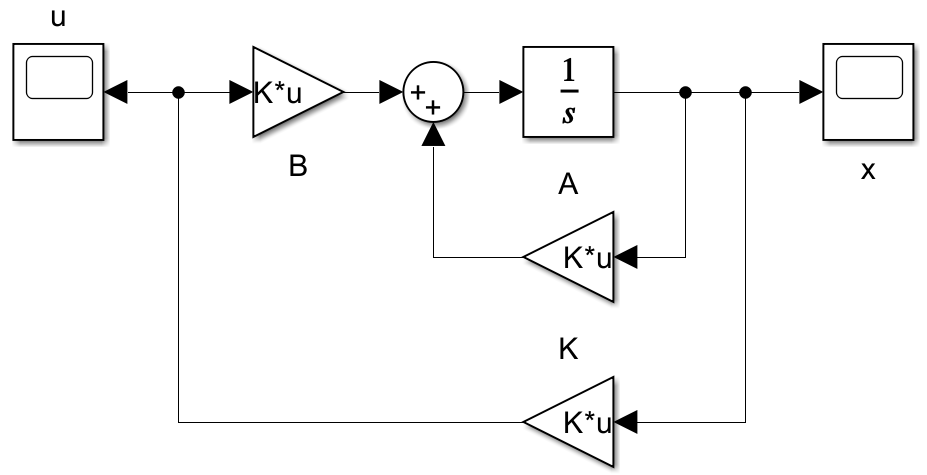
\includegraphics[scale=0.5]{scheme_task1.png}
        \captionsetup{skip=0pt}
        \caption{Схема моделирования системы, замкнутой регулятором}
        \label{fig:scheme_task1}
    \end{figure}


    \subsection{Достижимые спектры}
    Рассмотрим предложенные спектры замкнутой системы $\left(A+BK\right)$ и определим, какие из них достижимы.
    Мы хотим, чтобы матрица $\left(A+BK\right)$ была устойчивой, то есть все ее собственные числа имели
    отрицательную действительную часть. В нашем случае комплексная пара $\lambda_{2,3}$ являются неустойчивыми,
    но управляемыми -- их можно переместить в устойчивую область (подобрать любые числа, меньшие нуля). Собственное
    число $\lambda_1=-2$ устойчивое, но неуправляемое -- его не получится переместить куда-либо. Это означает, что
    спектр $\sigma\left(A+BK\right)$ должен содержать это неуправляемое число, иначе регулятор не будет выполнять свою
    функцию, мы потеряем собственное число матрицы $A$. Таким образом, желаемый спектр должен содержать все неуправляемые (но устойчивые)
    собственные числа матрицы $A$, при этом остальные числа могут быть любыми, но устойчивыми. Важно уточнить, что
    если некоторое собственное число матрицы $A$ неустойчиво и неуправляемо, то система не стабилизируема -- модальный
    регулятор применить не получится.


    Исходя из наших рассуждений выше, достижимыми будут следующие спектры замкнутой системы
    $$
    \sigma\left(A+BK\right)= 
    \left[ 
      \begin{gathered} 
        \left\{-2,-2,-2\right\}, \\ 
        \left\{-2,-20,-200\right\},\\
        \left\{-2,-2\pm6i\right\};
      \end{gathered} 
\right.
    $$
    Остальные спектры не содержат неуправляемое собственное число $\lambda_1=-2$.


    \subsection{Матрица регулятора}
    Для каждого из достижимых спектров, определенных в предыдущем пункте, найдем
    соответствующие матрицы регулятора $K$, приводящие спектр замкнутой системы
    к желаемому.


    Рассмотрим спектр $\sigma\left(A+BK\right)=\left\{-2,-2,-2\right\}$. Запишем полином
    Ньютона третьего порядка с $\omega_0=1$
    $$
    \left(\lambda+2\right)^3=\lambda^3+6\lambda^2+12\lambda+8
    $$
    Составим матрицу $\Gamma_1$ в канонической наблюдаемой форме по коэффициентам найденного полинома
    $$
\Gamma_1=\begin{bmatrix}
    0 &1 &0\\
    0 &0 &1\\
    -8 &-12 &-6
\end{bmatrix}
    $$
    Подберем $Y_1$ такой, чтобы пара $\left(Y_1,\Gamma_1\right)$ была наблюдаема. Проверим, вычислив ранг
    матрицы наблюдаемости
    $$
    Y_1=\begin{bmatrix}
        1 &0 &0
    \end{bmatrix},\ \text{rank}\begin{bmatrix}
        Y_1\\ Y_1\Gamma_1\\ Y_1\Gamma_1^2
    \end{bmatrix}=\text{rank}\begin{bmatrix}
    1     &0     &0\\
     0     &1     &0\\
     0     &0     &1
    \end{bmatrix}=3;
    $$
    Теперь, используя пакет \texttt{cvx} в \texttt{MATLAB}, вычислим матрицу $P_1\in\mathbb{R}^{3\times3}$
    как решение уравнения Сильвестра
    $$AP_1-P_1\Gamma_1=BY_1$$
    $$\begin{bmatrix}
        5 &2 &7\\
        2 &1 &2\\
        -2 &-3 &-4
    \end{bmatrix}\begin{bmatrix}
        p_1 &p_2 &p_3\\
        p_4 &p_5 &p_6\\
        p_7 &p_8 &p_9
    \end{bmatrix}-\begin{bmatrix}
        p_1 &p_2 &p_3\\
        p_4 &p_5 &p_6\\
        p_7 &p_8 &p_9
    \end{bmatrix}\begin{bmatrix}
        0 &1 &0\\
        0 &0 &1\\
        -8 &-12 &-6
    \end{bmatrix}=\begin{bmatrix}
        3\\
        1\\
        -1
    \end{bmatrix}\begin{bmatrix}
        1 &0 &0
    \end{bmatrix},$$
    $$
    P_1=\begin{bmatrix}
    0.4455   &-0.0701   &-0.0288\\
   -0.0759   &-0.1036   &-0.0181\\
    0.1649    &0.1926    &0.0404
    \end{bmatrix};
    $$
    Далее вычислим матрицу регулятора $K_1\in\mathbb{R}^{3\times3}$ по формуле
    $$K_1=-Y_1P_1^{-1},$$
    $$K_1=\begin{bmatrix}
        -1.800   &-7.043   &-4.443
    \end{bmatrix};$$
    Повторим шаги для нахождения остальных $K_i$. Рассмотрим спектры $$\sigma\left(A+BK\right)=\left\{-2,-20,-200\right\},\ \sigma\left(A+BK\right)=\left\{-2,-2\pm6i\right\};$$
    Найдем их полиномы
    $$\left(\lambda+2\right)\left(\lambda+20\right)\left(\lambda+200\right)=\lambda^3+222\lambda^2+4440\lambda+8000,$$
    $$\left(\lambda+2\right)\left(\lambda+2-6i\right)\left(\lambda+2+6i\right)=\lambda^3+6\lambda^2+48\lambda+80;$$
    Аналогично запишем матрицы $\Gamma_i$
    $$\Gamma_2=\begin{bmatrix}
        0 &1 &0\\
        0 &0 &1\\
        -8000 &-4440 &-222
    \end{bmatrix},\ \Gamma_3=\begin{bmatrix}
        0 &1 &0\\
        0 &0 &1\\
        -80 &-48 &-6
    \end{bmatrix};$$
    Подберем $Y_i$ и выполним проверку ранга
    $$
    Y_{2,3}=Y_1=\begin{bmatrix}
        1 &0 &0
    \end{bmatrix}=Y,\
    \text{rank}\begin{bmatrix}
        Y\\
        Y\Gamma_2\\
        Y\Gamma_2^2
    \end{bmatrix}=\text{rank}\begin{bmatrix}
        Y\\
        Y\Gamma_3\\
        Y\Gamma_3^2
    \end{bmatrix}=\text{rank}\begin{bmatrix}
        1 &0 &0\\
        0 &1 &0\\
        0 &0 &1
    \end{bmatrix}=3;
    $$
    Найдем $P_{2,3}$ и $K_{2,3}$ тем же способом
    $$
    P_2=\begin{bmatrix}
    0.2259    &0.0053    &0.0000\\
    0.0612    &0.0012    &0.0000\\
    0.2253    &0.0146    &0.0001
    \end{bmatrix},\ P_3=\begin{bmatrix}
    0.2546    &0.0351   &-0.0026\\
    0.0744    &0.0055   &-0.0012\\
    0.2550    &0.0275    &0.0094
    \end{bmatrix},
    $$
    $$
    K_2=\begin{bmatrix}
        754.2 &-2553.6 &-67.0
    \end{bmatrix},\ K_3=\begin{bmatrix}
        5.4000  &-25.9424   &-1.7424
    \end{bmatrix};
    $$


    \subsection{Корректность синтеза регулятора}
    Определим собственные числа каждой матрицы замкнутой системы $\left(A+BK_i\right)$ и
    сравним с соответствующими желаемыми спектрами
    $$
    \sigma\left(A+BK_1\right)=\sigma\begin{bmatrix}
    -0.400  &-19.129   &-6.329\\
    0.200   &-6.043   &-2.443\\
   -0.200    &4.043    &0.443
    \end{bmatrix}=\left\{-2,-2,-2\right\},
    $$
    $$
    \sigma\left(A+BK_2\right)=\sigma\begin{bmatrix}
    2267.6   &-7658.7   &-193.9\\
    756.2   &-2552.6   &-65.0\\
   -756.2    &2550.6    &63.0
    \end{bmatrix}=\left\{-2,-20,-200\right\},
    $$
    $$
    \sigma\left(A+BK_3\right)=\sigma\begin{bmatrix}
    21.2000  &-75.8273    &1.7727\\
    7.4000  &-24.9424    &0.2576\\
   -7.4000   &22.9424   &-2.2576
    \end{bmatrix}=\left\{-2,-2\pm6i\right\};
    $$
    Видим, что спектры совпадают с желаемыми -- регулятор синтезирован корректно.

    % pos 1636,387,726,312
    \subsection{Компьютерное моделирование}
    Для компьютерного моделирования воспользуемся схемой \texttt{SIMULINK},
    представленной на рис. \ref{fig:scheme_task1}.
    Зададим в интегратор начальное условие $x(0)=\begin{bmatrix}
        1 &1 &1
    \end{bmatrix}^T$
    \begin{figure}[H]
        \centering
        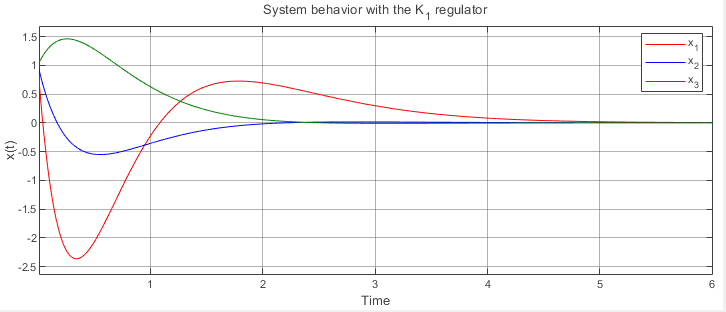
\includegraphics[scale=0.7]{1task_xt_k1.png}
        \captionsetup{skip=0pt}
        \caption{График $x(t)$ для $K_1$}
        \label{fig:1task_xt_k1}
    \end{figure}
    \begin{figure}[H]
        \centering
        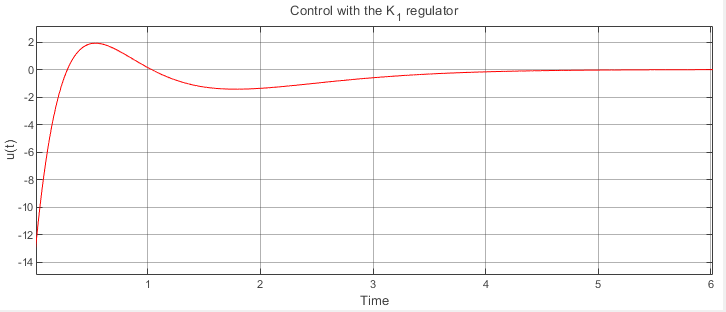
\includegraphics[scale=0.7]{1task_ut_k1.png}
        \captionsetup{skip=0pt}
        \caption{График $u(t)$ для $K_1$}
        \label{fig:1task_ut_k1}
    \end{figure}
    \newpage
    \vspace*{5mm}
    \begin{figure}[H]
        \centering
        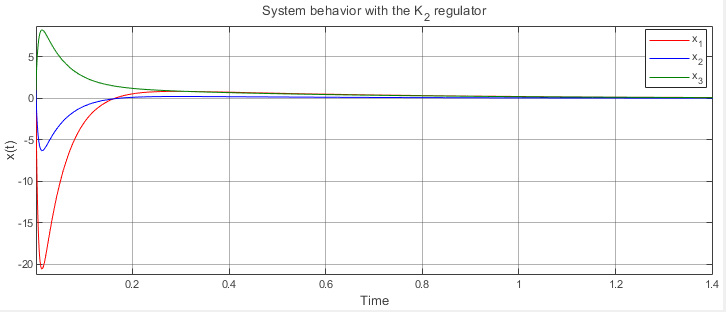
\includegraphics[scale=0.7]{1task_xt_k2.png}
        \captionsetup{skip=0pt}
        \caption{График $x(t)$ для $K_2$}
        \label{fig:1task_xt_k2}
    \end{figure}
    \begin{figure}[H]
        \centering
        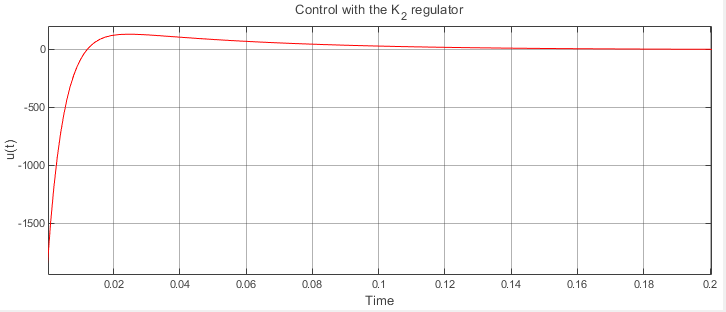
\includegraphics[scale=0.7]{1task_ut_k2.png}
        \captionsetup{skip=0pt}
        \caption{График $u(t)$ для $K_2$}
        \label{fig:1task_ut_k2}
    \end{figure}
    \begin{figure}[H]
        \centering
        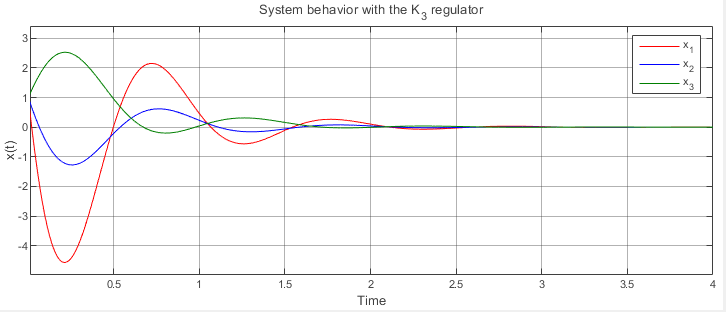
\includegraphics[scale=0.7]{1task_xt_k3.png}
        \captionsetup{skip=0pt}
        \caption{График $x(t)$ для $K_3$}
        \label{fig:1task_xt_k3}
    \end{figure}
    \begin{figure}[H]
        \centering
        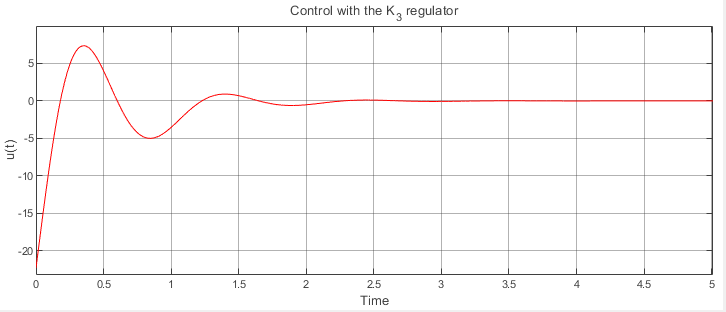
\includegraphics[scale=0.7]{1task_ut_k3.png}
        \captionsetup{skip=0pt}
        \caption{График $u(t)$ для $K_3$}
        \label{fig:1task_ut_k3}
    \end{figure}


    \subsection{Сравнение результатов}
    Сопоставим полученные результаты компьютерного моделирования для рассмотренных спектров,
    оценим возможные сравнительные преимущества и недостатки каждого из них.


    На каждом рисунке система $x(t)$ стабилизировалась -- все координаты пришли в ноль, выходя из 1.
    Управления $u(t)$ сошлись к нулю -- регуляторы выполнили свою задачу и больше не требуют
    активного управления.
    

    На рис. \ref{fig:1task_ut_k1} видим, что управление $u(t)$ достаточно плавное,
    имеет небольшое перерегулирование в сравнении с другими графиками.
    На рис. \ref{fig:1task_xt_k1} система $x(t)$ ожидаемо медленно и плавно затухает.


    На рис. \ref{fig:1task_xt_k2} наблюдаем быстрое стабилизирование системы, однако при
    этом присутствуют большие начальные отклонения. В сравнении с другими графиками имеется
    ожидаемо наибольшее перерегулирование (см. рис. \ref{fig:1task_ut_k2}).
    Получили достаточно агрессивный регулятор.


    На рис. \ref{fig:1task_xt_k3} система, вследствие наличия комплексных собственных чисел,
    приобрела сравнительно небольшие осцилляции. По скорости затухания колебаний результат получился средним
    (быстрее, чем $K_1$; медленнее, чем $K_2$). Система выглядит менее предсказуемо в сравнении с остальными результатами.


    \subsection{Вывод}
    В ходе выполнения задания мы выяснили, что система не полностью управляема, но стабилизируема.
    Мы нашли достижимые спектры по принципу наличия в них неуправляемых (но устойчивых) собственных чисел
    матрицы $A$. Мы вычислили матрицы регулятора, убедились в корректности синтеза каждого регулятора, после чего
    провели компьютерное моделирование. В ходе сравнения результатов было выяснено, что при маленьких собственных
    числах в спектре система медленно и плавно затухает со сравнительно небольшим перерегулированием. При больших
    по модулю собственных числах система быстро стабилизируется, но имеет сравнительно большое перерегулирование.
    Наличие комплексных собственных чисел создаст некоторые осцилляции в системе, из-за чего она может быть менее
    предсказуема. При этом скорость затухания системы выше, чем при небольших по модулю числах, принадлежащих множеству рациональных чисел.


    \section{Задание 2. Наблюдатель полного порядка}
    Рассмотрим систему
    $$
    \begin{cases}
        \dot{x}=Ax,\\
        y=Cx,
    \end{cases}\ A=\begin{bmatrix}
        0 &1 &0 &1\\
        -26 &-7 &20 &-11\\
        0 &1 &-1 &2\\
        16 &4 &-14 &8
    \end{bmatrix},\ C=\begin{bmatrix}
        -1 &0 &1 &-1
    \end{bmatrix},
    $$
    $$
    \sigma\left(A+LC\right)= 
    \left[ 
      \begin{gathered} 
        \left\{-2,-2,-2, -2\right\}, \\ 
        \left\{-2,-20,-200, -2000\right\},\\
        \left\{-2\pm3i,-2\pm4i\right\};
      \end{gathered} 
\right.
    $$


    \subsection{Наблюдаемость и обнаруживоемость}
    Найдем собственные числа матрицы $A$.
    Программа для вычислений в \texttt{MATLAB} находится в приложении
    2 на листинге \ref{task2}
    $$
    \det{\left[\lambda I-A\right]}=\begin{vmatrix}
        \lambda &-1 &0 &-1\\
        26 &\lambda+7 &-20 &11\\
        0 &-1 &\lambda+1 &-2\\
        -16 &-4 &14 &\lambda-8
    \end{vmatrix}=0,
    $$
    $$
    \sigma\left(A\right)=\left\{\pm2i,\pm i\right\};
    $$
    Все собственные числа комплексные и имеют нулевую действительную часть.
    Следовательно, они все устойчивые, но не асимптотически. То есть в системе будут незатухающие колебания.
    Перейдем к вещественной жордановой форме системы, чтобы определить наблюдаемость каждого собственного числа,
    а далее сделать выводы о наблюдаемости и обнаруживоемости системы
    $$
    A=P_{re}J_{re}P_{re}^{-1}=\begin{bmatrix}
    -0.5 &-0.5    &0.5   &-0.5\\
    0   &-1   &-0.5    &0.5\\
    0   &-1    &1   &-0.5\\
    1   &0    &1    &0
    \end{bmatrix}\begin{bmatrix}
    0    &2   &0    &0\\
   -2   &0    &0   &0\\
    0   &0    &0    &1\\
   0   &0   &-1   &0
    \end{bmatrix}\begin{bmatrix}
    -8   &-2    &6   &-3\\
    2   &-0   &-2    &1\\
    8    &2   &-6    &4\\
   12    &4  &-10    &6
    \end{bmatrix},
    $$
    $$
    C_{Jre}=CP_{re}=\begin{bmatrix}
        -1 &0 &1 &-1
    \end{bmatrix}\begin{bmatrix}
        -0.5 &-0.5    &0.5   &-0.5\\
        0   &-1   &-0.5    &0.5\\
        0   &-1    &1   &-0.5\\
        1   &0    &1    &0
    \end{bmatrix}=\begin{bmatrix}
        -0.5   &-0.5   &-0.5         &0
    \end{bmatrix};
    $$
    Итого имеем
    $$
    J_{re}=\begin{bmatrix}
        0    &2   &0    &0\\
       -2   &0    &0   &0\\
        0   &0    &0    &1\\
       0   &0   &-1   &0
    \end{bmatrix},\ C_{Jre}=\begin{bmatrix}
        -0.5   &-0.5   &-0.5         &0
    \end{bmatrix};
    $$
    Все жордановы клетки относятся к различным собственным числам. Все собственные числа, кроме
    $\lambda_4$, наблюдаемы, так как соответствующие им элементы матрицы выходов $C_{Jre}$
    не равны нулю. Из этого нельзя сделать вывод, что система полностью наблюдаема. Достаточное
    условие полной наблюдаемости нашей системы -- не равенство нулю $\left[\text{первого или второго}\right]$
    и $\left[\text{третьего или четвертого}\right]$ элементов матрицы $C_{Jre}$. Так как условие
    выполняется, то система полностью наблюдаема, а значит, и обнаруживаема.


    \subsection{Схема моделирования системы с наблюдателем состояния}
    Построим в \texttt{SIMULINK} схему моделирования системы с наблюдателем состояния
    $\dot{\hat{x}}=A\hat{x}+L\left(C\hat{x}-y\right)$
    \begin{figure}[H]
        \centering
        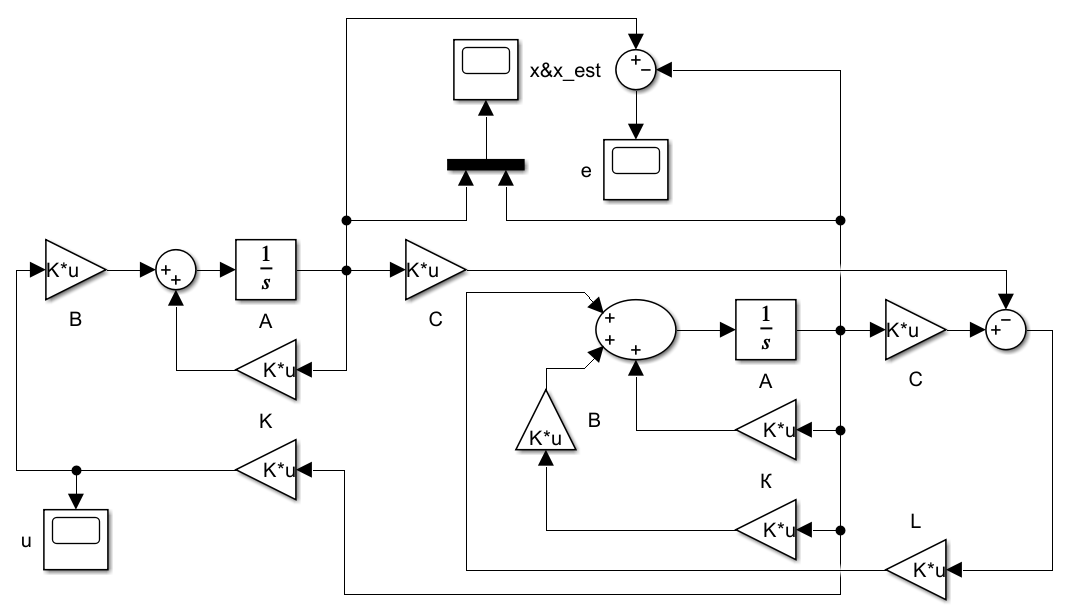
\includegraphics[scale=0.45]{scheme_task2.png}
        \captionsetup{skip=0pt}
        \caption{Схема моделирования системы с наблюдателем состояния}
        \label{fig:scheme_task2}
    \end{figure}
    \noindent Через один \texttt{Scope} отслеживаем сигналы $x(t)\text{ и }\hat{x}(t)$ на одном графике,
    через другой ошибку наблюдателя (невязку) $e(t)=x(t)-\hat{x}(t)$.


    \subsection{Матрица коррекции наблюдателя}
    Для каждого из предложенных спектров найдем матрицы коррекции наблюдателя $L$, обеспечивающих
    соответствующий желаемый спектр. Аналогично первому заданию составим полиномы
    \begin{align*}
    &\left(\lambda+2\right)^4=\lambda^4+8\lambda^3+24\lambda^2+32\lambda+16,\\
    &\left(\lambda+2\right)\left(\lambda+20\right)\left(\lambda+200\right)\left(\lambda+2000\right)=
    \lambda^4+2222\lambda^3+448440\lambda^2+8888000\lambda+16000000,\\
    &\left(\lambda+2-3i\right)\left(\lambda+2+3i\right)\left(\lambda+2-4i\right)\left(\lambda+2+4i\right)=
    \lambda^4+8\lambda^3+49\lambda^2+132\lambda+260;
    \end{align*}
    Запишем матрицы $\Gamma_i$
    $$
    \Gamma_1=\begin{bmatrix}
        0 &1 &0 &0\\
        0 &0 &1 &0\\
        0 &0 &0 &1\\
        -16 &-32 &-24 &-8
    \end{bmatrix},\ \Gamma_2=\begin{bmatrix}
        0 &1 &0 &0\\
        0 &0 &1 &0\\
        0 &0 &0 &1\\
        -16000000 &-8888000 &-448440 &-2222
    \end{bmatrix},
    $$
    $$
    \Gamma_3=\begin{bmatrix}
        0 &1 &0 &0\\
        0 &0 &1 &0\\
        0 &0 &0 &1\\
        -260 &-132 &-49 &-8
    \end{bmatrix};
    $$
    Все матрицы $\Gamma_i$ составлены по одинаковому принципу, поэтому подберем единый $Y$ такой, чтобы
    пары $\left(Y,\Gamma_i\right)$ были управляемы. Проверим, вычислив ранги матриц управляемости $U_i$
    $$
    Y=\begin{bmatrix}
        1\\
        0\\
        0\\
        0
    \end{bmatrix},\ U_i=\begin{bmatrix}
        Y &\Gamma_iY &\Gamma_i^2Y &\Gamma_i^3Y
    \end{bmatrix},
    $$
    $$
    \text{rank}\begin{bmatrix}Y &\Gamma_1Y &\Gamma_1^2Y &\Gamma_1^3Y\end{bmatrix}=\text{rank}\begin{bmatrix}
    1     &0     &0     &0\\
    0     &0     &0   &-16\\
    0     &0   &-16   &128\\
    0   &-16   &128  &-640
    \end{bmatrix}=4,
    $$
    $$
    \text{rank}\begin{bmatrix}Y &\Gamma_2Y &\Gamma_2^2Y &\Gamma_2^3Y\end{bmatrix}=\text{rank}\left[10^{13}\cdot\begin{bmatrix}
        0.0000         &0.0000         &0.0000         &0.0000\\
        0.0000         &0.0000         &0.0000   &0.0000\\
        0.0000         &0.0000   &0.0000    &0.0036\\
        0.0000   &0.0000    &0.0036   &-7.1822
    \end{bmatrix}\right]=4,
    $$
    $$
    \text{rank}\begin{bmatrix}Y &\Gamma_3Y &\Gamma_3^2Y &\Gamma_3^3Y\end{bmatrix}=\text{rank}\begin{bmatrix}
        1           &0           &0           &0\\
        0           &0           &0        &-260\\
        0           &0        &-260        &2080\\
        0        &-260        &2080       &-3900
    \end{bmatrix}=4;
    $$
    Используя пакет \texttt{cvx} в \texttt{MATLAB}, вычилим матрицы $Q_i\in\mathbb{R}^{4\times4}$ как решения уравнения Сильвестра
    $$
    \Gamma_iQ_i-Q_iA=YC
    $$
    После чего вычислим $L_i\in\mathbb{R}^{4\times1}$ по формуле
    $$
    L_i=Q_i^{-1}Y
    $$
    Получаем следующие результаты
    $$
    Q_1=\begin{bmatrix}
    -7.7426   &-2.3690    &6.5528   &-3.5588\\
    3.6532    &1.1580   &-3.1096    &1.9516\\
    1.1176    &0.2440   &-1.0528    &0.3088\\
   -1.4032   &-0.4080    &1.6096   &-1.2016
    \end{bmatrix},\ L_1=\begin{bmatrix}
    10.3333\\
  -21.0000\\
    7.6667\\
    5.3333
    \end{bmatrix},
    $$
    $$
    Q_2=\begin{bmatrix}
    -1.7989   &-0.5605    &1.4628   &-0.6220\\
    3.6220    &1.0996   &-2.9656    &1.3166\\
   -7.5251   &-1.7746    &6.5261   &-3.8724\\
  -15.8185   &-4.0663   &12.1953   &-5.9314
    \end{bmatrix},\ L_2=10^6\cdot\begin{bmatrix}
        0.7378\\
    7.5493\\
    6.0674\\
    5.3319
    \end{bmatrix},
    $$
    $$
    Q_3=\begin{bmatrix}
    -1.4397   &-0.4741    &1.0517   &-0.3017\\
    6.5000    &1.7241   &-5.3103    &2.4655\\
   -5.3793   &-1.0172    &5.2759   &-3.3621\\
  -27.3448   &-6.4310   &21.4483  &-10.5345
    \end{bmatrix},\ L_3=\begin{bmatrix}
        4.0000\\
   76.0000\\
   58.6667\\
   62.6667
    \end{bmatrix};
    $$


    \subsection{Корректность синтеза наблюдателя}
    Определим собственные числа матриц наблюдателя $\left(A+L_iC\right)$
    и сравним с соответствующими желаемыми спектрами
    $$
    \sigma\left(A+L_1C\right)=\sigma\begin{bmatrix}
    -10.3333    &1.0000   &10.3333   &-9.3333\\
   -5.0000   &-7.0000   &-1.0000   &10.0000\\
   -7.6667    &1.0000    &6.6667   &-5.6667\\
   10.6667    &4.0000   &-8.6667    &2.6667
    \end{bmatrix}=
    \left\{
    \begin{matrix}
        -2.0017\\
    -2.0000 + 0.0017i\\
    -2.0000 - 0.0017i\\
    -1.9983
    \end{matrix}\right\},
    $$
    $$
    \sigma\left(A+L_2C\right)=\sigma\left[10^6\cdot\begin{bmatrix}
    -0.7378    &0.0000    &0.7378   &-0.7378\\
   -7.5494   &0.0000    &7.5494   &-7.5494\\
   -6.0674    &0.0000    &6.0674   &-6.0674\\
   -5.3318    &0.0000    &5.3318   &-5.3318
    \end{bmatrix}\right]=\left\{\begin{matrix}
    -2000\\
   -200\\
   -2\\
   -20
    \end{matrix}\right\},
    $$
    $$
    \sigma\left(A+L_3C\right)=\sigma\begin{bmatrix}
        -4.0000    &1.0000    &4.0000   &-3.0000\\
 -102.0000   &-7.0000   &96.0000  &-87.0000\\
  -58.6667    &1.0000   &57.6667  &-56.6667\\
  -46.6667    &4.0000   &48.6667  &-54.6667
    \end{bmatrix}=\left\{\begin{matrix}
        -2\pm4i\\
        -2\pm3i
    \end{matrix}\right\};
    $$
    Отклонение в $0.085\%$ для $L_1$ будем считать погрешностью вычислений в \texttt{MATLAB}.
    Остальные спектры совпали с желаемыми. Наблюдатель синтезирован корректно.


    \subsection{Компьютерное моделирование}
    Для компьютерного моделирования воспользуемся схемой \texttt{SIMULINK},
    представленной на рис. \ref{fig:scheme_task2}. Зададим в интеграторы
    такие начальные условия:
    для системы $x(0)=\begin{bmatrix}
        1 &1 &1 &1
    \end{bmatrix}^T$, для наблюдателя $\hat{x}(0)=\begin{bmatrix}
        2 &0 &0 &-1
    \end{bmatrix}^T$. Также для одного из случаев приблизим график к началу времени $t$,
    чтобы убедиться в том, что каждая координата выходит из своего начального условия
    % L1
    \begin{figure}[H]
        \centering
        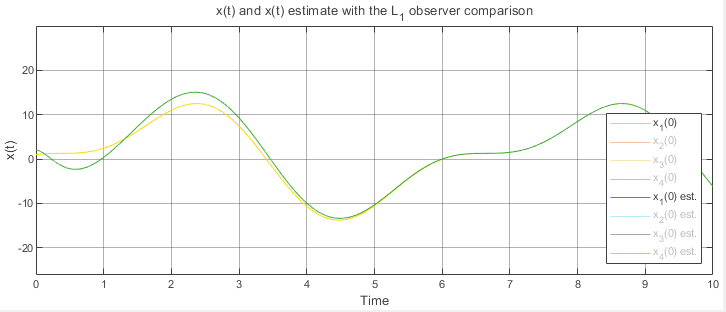
\includegraphics[scale=0.7]{2task_x1comp_L1.png}
        \captionsetup{skip=0pt}
        \caption{Графики $x_1(t),\hat{x}_1(t)$ для $L_1$}
        \label{fig:2task_x1comp_L1}
    \end{figure}
    \begin{figure}[H]
        \centering
        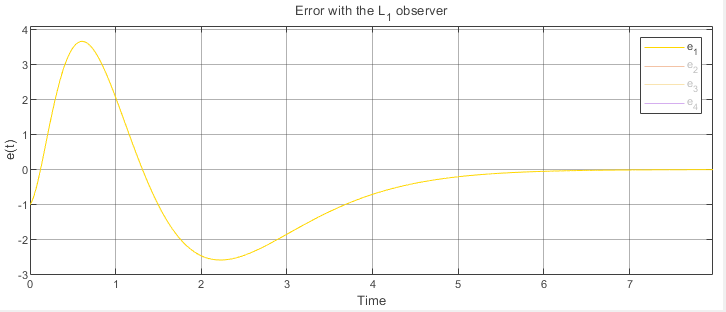
\includegraphics[scale=0.7]{2task_e1_L1.png}
        \captionsetup{skip=0pt}
        \caption{График $e_1(t)$ для $L_1$}
        \label{fig:2task_e1_L1}
    \end{figure}
    \newpage
    \vspace*{5mm}
    \begin{figure}[H]
        \centering
        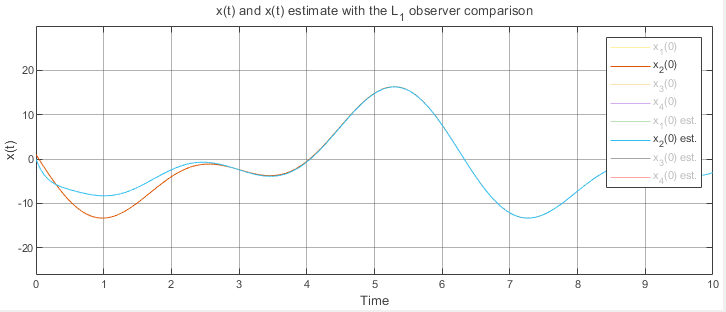
\includegraphics[scale=0.7]{2task_x2comp_L1.png}
        \captionsetup{skip=0pt}
        \caption{Графики $x_2(t),\hat{x}_2(t)$ для $L_1$}
        \label{fig:2task_x2comp_L1}
    \end{figure}
    \begin{figure}[H]
        \centering
        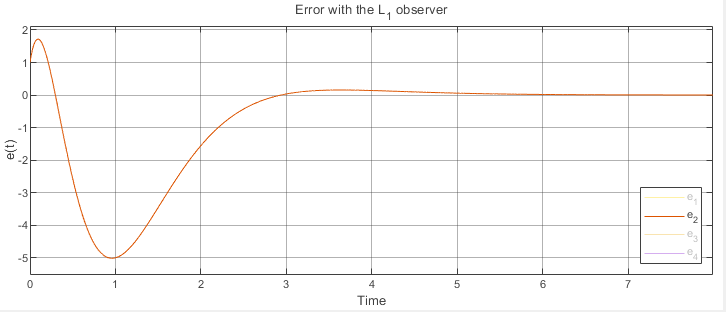
\includegraphics[scale=0.7]{2task_e2_L1.png}
        \captionsetup{skip=0pt}
        \caption{График $e_2(t)$ для $L_1$}
        \label{fig:2task_e2_L1}
    \end{figure}
    \begin{figure}[H]
        \centering
        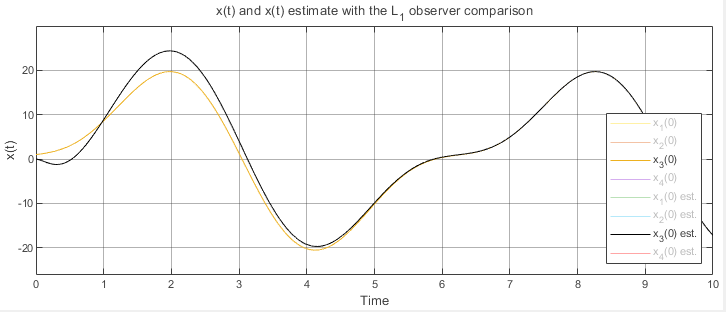
\includegraphics[scale=0.7]{2task_x3comp_L1.png}
        \captionsetup{skip=0pt}
        \caption{Графики $x_3(t),\hat{x}_3(t)$ для $L_1$}
        \label{fig:2task_x3comp_L1}
    \end{figure}
    \newpage
    \vspace*{5mm}
    \begin{figure}[H]
        \centering
        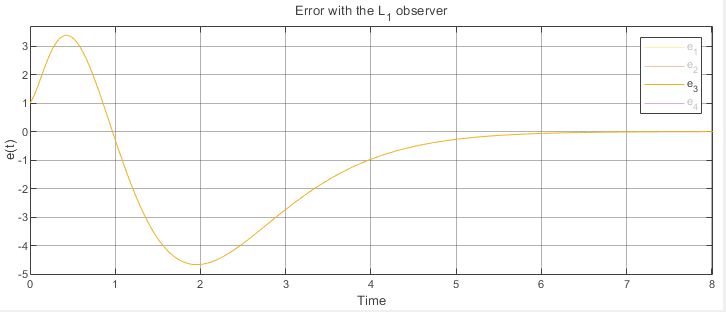
\includegraphics[scale=0.7]{2task_e3_L1.png}
        \captionsetup{skip=0pt}
        \caption{График $e_3(t)$ для $L_1$}
        \label{fig:2task_e3_L1}
    \end{figure}
    \begin{figure}[H]
        \centering
        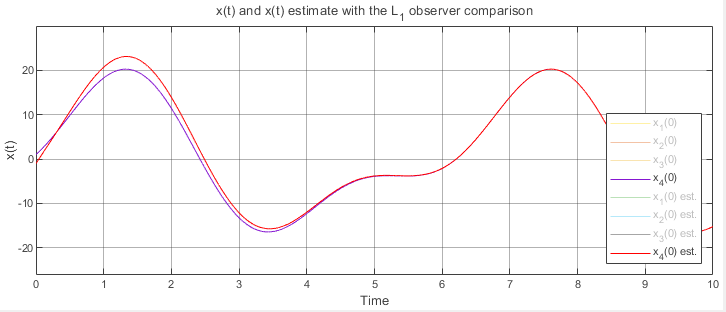
\includegraphics[scale=0.7]{2task_x4comp_L1.png}
        \captionsetup{skip=0pt}
        \caption{Графики $x_4(t),\hat{x}_4(t)$ для $L_1$}
        \label{fig:2task_x4comp_L1}
    \end{figure}
    \begin{figure}[H]
        \centering
        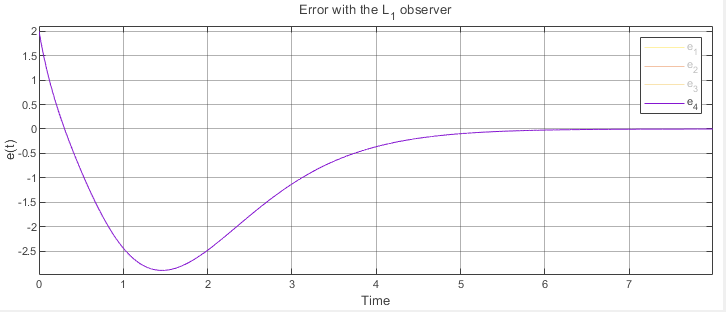
\includegraphics[scale=0.7]{2task_e4_L1.png}
        \captionsetup{skip=0pt}
        \caption{График $e_4(t)$ для $L_1$}
        \label{fig:2task_e4_L1}
    \end{figure}
    % L2
    \newpage
    \vspace*{5mm}
    \begin{figure}[H]
        \centering
        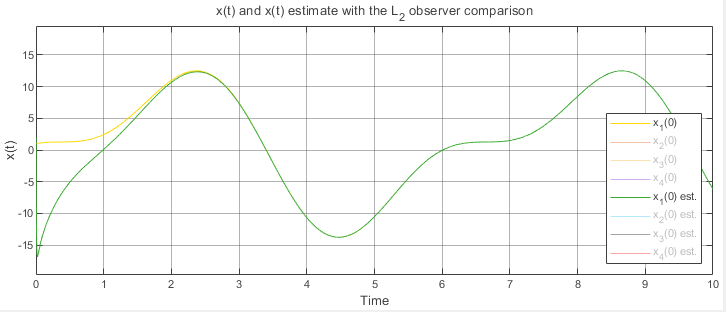
\includegraphics[scale=0.7]{2task_x1comp_L2.png}
        \captionsetup{skip=0pt}
        \caption{Графики $x_1(t),\hat{x}_1(t)$ для $L_2$}
        \label{fig:2task_x1comp_L2}
    \end{figure}
    \begin{figure}[H]
        \centering
        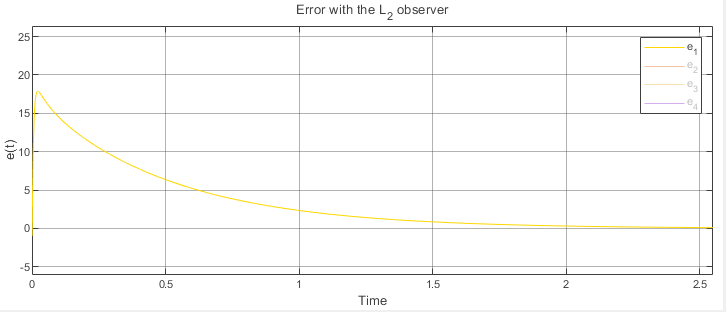
\includegraphics[scale=0.7]{2task_e1_L2.png}
        \captionsetup{skip=0pt}
        \caption{График $e_1(t)$ для $L_2$}
        \label{fig:2task_e1_L2}
    \end{figure}
    \begin{figure}[H]
        \centering
        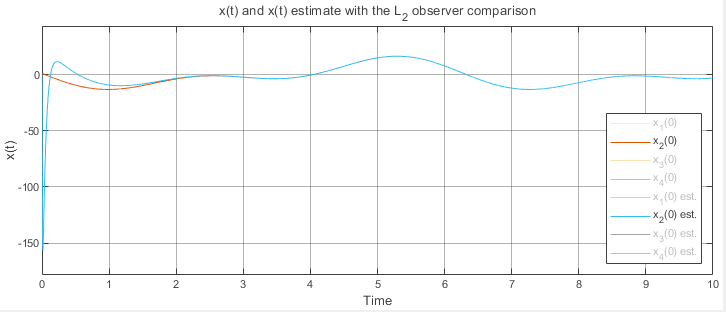
\includegraphics[scale=0.7]{2task_x2comp_L2.png}
        \captionsetup{skip=0pt}
        \caption{Графики $x_2(t),\hat{x}_2(t)$ для $L_2$}
        \label{fig:2task_x2comp_L2}
    \end{figure}
    \newpage
    \vspace*{5mm}
    \begin{figure}[H]
        \centering
        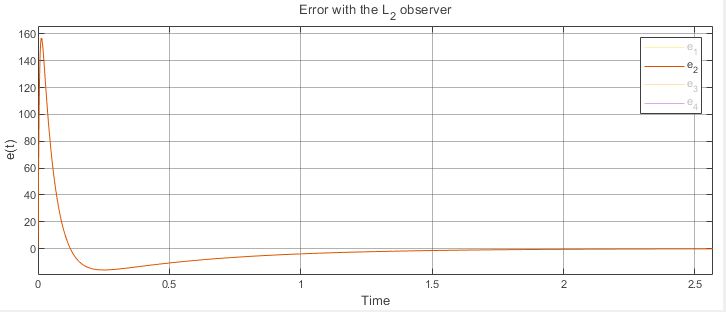
\includegraphics[scale=0.7]{2task_e2_L2.png}
        \captionsetup{skip=0pt}
        \caption{График $e_2(t)$ для $L_2$}
        \label{fig:2task_e2_L2}
    \end{figure}
    \begin{figure}[H]
        \centering
        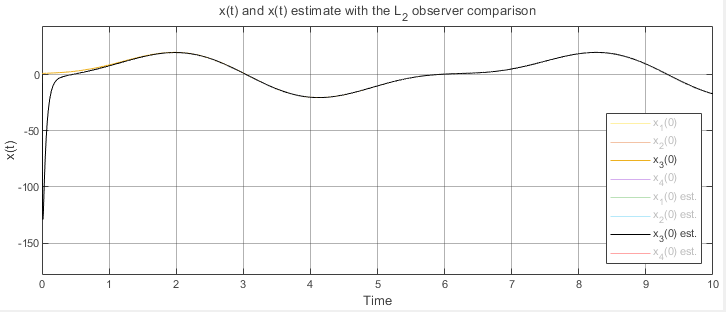
\includegraphics[scale=0.7]{2task_x3comp_L2.png}
        \captionsetup{skip=0pt}
        \caption{Графики $x_3(t),\hat{x}_3(t)$ для $L_2$}
        \label{fig:2task_x3comp_L2}
    \end{figure}
    \begin{figure}[H]
        \centering
        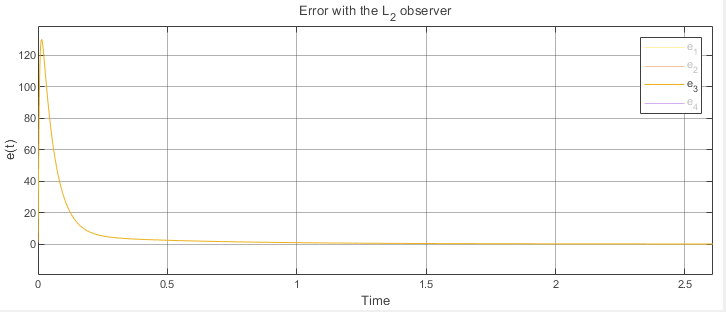
\includegraphics[scale=0.7]{2task_e3_L2.png}
        \captionsetup{skip=0pt}
        \caption{График $e_3(t)$ для $L_2$}
        \label{fig:2task_e3_L2}
    \end{figure}
    \newpage
    \vspace*{5mm}
    \begin{figure}[H]
        \centering
        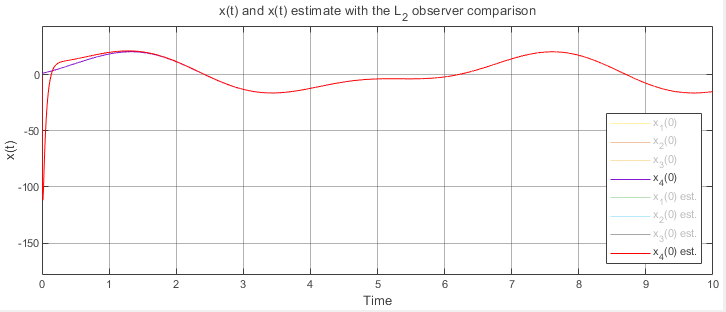
\includegraphics[scale=0.7]{2task_x4comp_L2.png}
        \captionsetup{skip=0pt}
        \caption{Графики $x_4(t),\hat{x}_4(t)$ для $L_2$}
        \label{fig:2task_x4comp_L2}
    \end{figure}
    \begin{figure}[H]
        \centering
        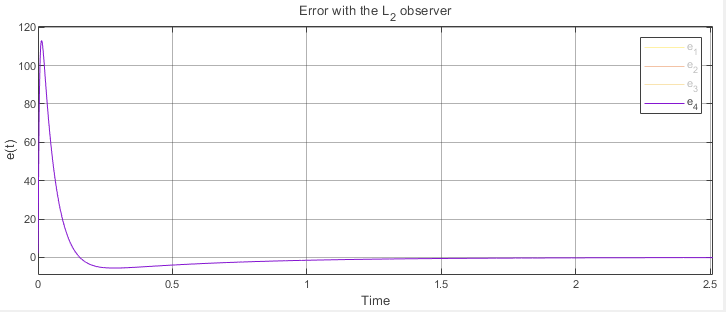
\includegraphics[scale=0.7]{2task_e4_L2.png}
        \captionsetup{skip=0pt}
        \caption{График $e_4(t)$ для $L_2$}
        \label{fig:2task_e4_L2}
    \end{figure}
    % L3
    \begin{figure}[H]
        \centering
        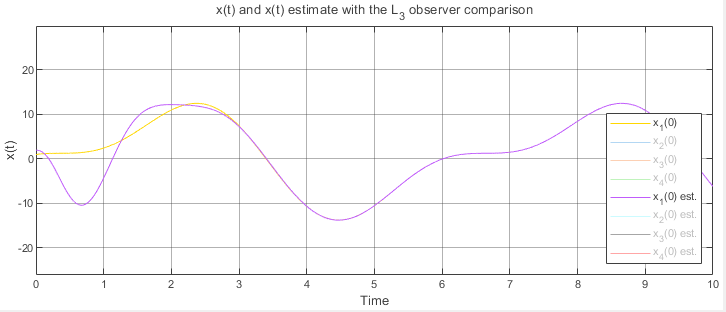
\includegraphics[scale=0.7]{2task_x1comp_L3.png}
        \captionsetup{skip=0pt}
        \caption{Графики $x_1(t),\hat{x}_1(t)$ для $L_3$}
        \label{fig:2task_x1comp_L3}
    \end{figure}
    \newpage
    \vspace*{5mm}
    \begin{figure}[H]
        \centering
        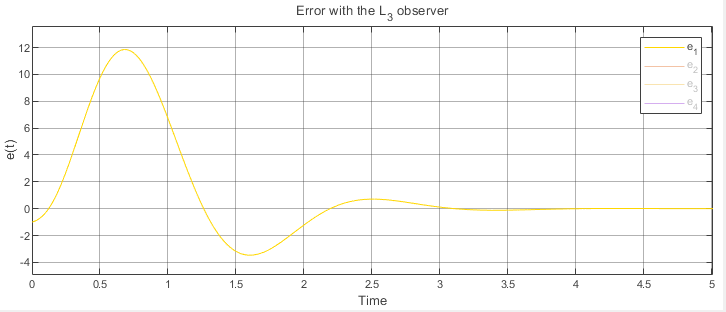
\includegraphics[scale=0.7]{2task_e1_L3.png}
        \captionsetup{skip=0pt}
        \caption{График $e_1(t)$ для $L_3$}
        \label{fig:2task_e1_L3}
    \end{figure}
    \begin{figure}[H]
        \centering
        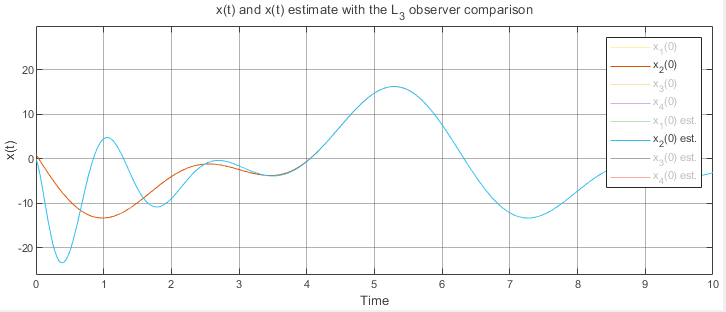
\includegraphics[scale=0.7]{2task_x2comp_L3.png}
        \captionsetup{skip=0pt}
        \caption{Графики $x_2(t),\hat{x}_2(t)$ для $L_3$}
        \label{fig:2task_x2comp_L3}
    \end{figure}
    \begin{figure}[H]
        \centering
        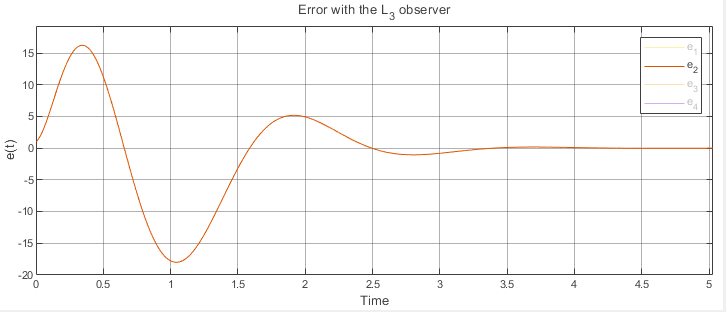
\includegraphics[scale=0.7]{2task_e2_L3.png}
        \captionsetup{skip=0pt}
        \caption{График $e_2(t)$ для $L_3$}
        \label{fig:2task_e2_L3}
    \end{figure}
    \newpage
    \vspace*{5mm}
    \begin{figure}[H]
        \centering
        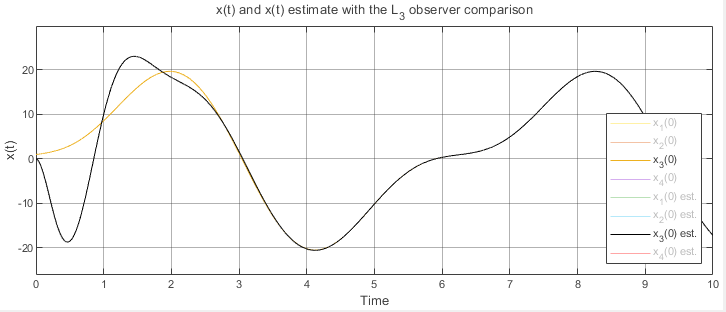
\includegraphics[scale=0.7]{2task_x3comp_L3.png}
        \captionsetup{skip=0pt}
        \caption{Графики $x_3(t),\hat{x}_3(t)$ для $L_3$}
        \label{fig:2task_x3comp_L3}
    \end{figure}
    \begin{figure}[H]
        \centering
        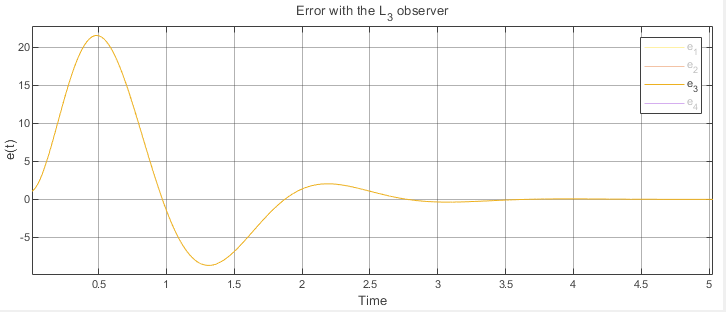
\includegraphics[scale=0.7]{2task_e3_L3.png}
        \captionsetup{skip=0pt}
        \caption{График $e_3(t)$ для $L_3$}
        \label{fig:2task_e3_L3}
    \end{figure}
    \begin{figure}[H]
        \centering
        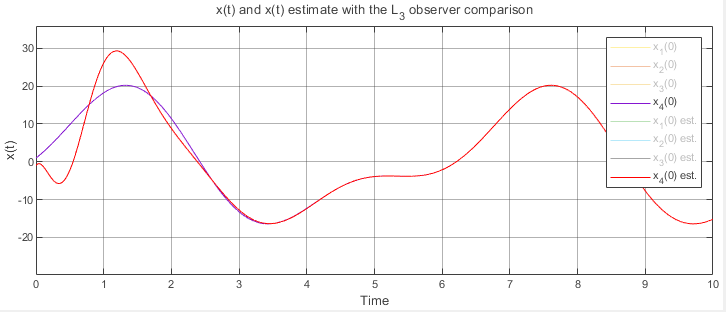
\includegraphics[scale=0.7]{2task_x4comp_L3.png}
        \captionsetup{skip=0pt}
        \caption{Графики $x_4(t),\hat{x}_4(t)$ для $L_3$}
        \label{fig:2task_x4comp_L3}
    \end{figure}
    \begin{figure}[H]
        \centering
        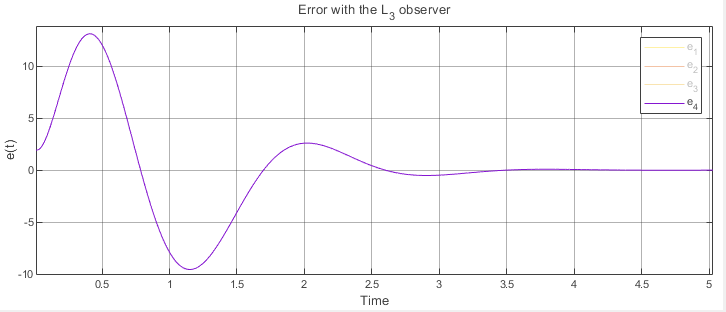
\includegraphics[scale=0.7]{2task_e4_L3.png}
        \captionsetup{skip=0pt}
        \caption{График $e_4(t)$ для $L_3$}
        \label{fig:2task_e4_L3}
    \end{figure}
    % L1 x0 check
    \begin{figure}[H]
        \centering
        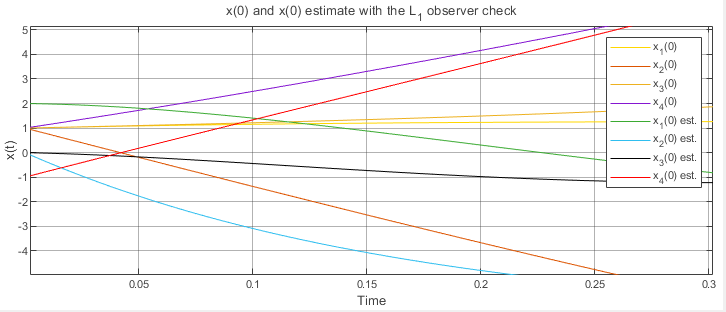
\includegraphics[scale=0.7]{2task_x0_L1.png}
        \captionsetup{skip=0pt}
        \caption{Проверка начальных условий (случай для $L_1$)}
        \label{fig:2task_x0_L1}
    \end{figure}


    \subsection{Сравнение результатов}
    Видим, как на каждом графике $x(t),\hat{x}(t)$ оценки координат сходятся к настоящим координатам -- наблюдатель
    выполняет свою работу верно. Например, на рис. \ref{fig:2task_x1comp_L1} \textbf{зеленая} оценка координаты $\hat{x}_1$ сходится
    к \textbf{желтой} истинной координате $x_1$ примерно за $t=7$. Ошибки ожидаемо стремятся к нулю. На рис. \ref{fig:2task_x0_L1}
    видим, что все координаты выходят из своих начальных условий.


    На рис. \ref{fig:2task_x1comp_L1}, \ref{fig:2task_x2comp_L1}, \ref{fig:2task_x3comp_L1}, \ref{fig:2task_x4comp_L1} видим, что примерно к $t=7$ каждая координата наблюдателя сошлась с исходными координатами.
    Ошибки на рис. \ref{fig:2task_e1_L1}, \ref{fig:2task_e2_L1}, \ref{fig:2task_e3_L1}, \ref{fig:2task_e4_L1} сравнительно небольшие, ожидаемо наибольшие в начале, далее плавно и медленно стремятся к нулю.
    Итого: плавное поведение наблюдателя с небольшой ошибкой, но медленное схождение к истинным координатам.


    На рис. \ref{fig:2task_x1comp_L2}, \ref{fig:2task_x2comp_L2}, \ref{fig:2task_x3comp_L2}, \ref{fig:2task_x4comp_L2} ситуация обратная -- наблюдатель быстро сводит координаты с координатами
    исходной системы (примерно за $t=3$), однако ошибки на рис. \ref{fig:2task_e1_L2}, \ref{fig:2task_e2_L2}, \ref{fig:2task_e3_L2}, \ref{fig:2task_e4_L2} ожидаемо сравнительно большие. На практике лучше всего
    соблюдать баланс между величиной ошибки и скоростью сходимости.


    На рис. \ref{fig:2task_x1comp_L3}, \ref{fig:2task_x2comp_L3}, \ref{fig:2task_x3comp_L3}, \ref{fig:2task_x4comp_L3} результат в целом схож с результатом для $L_1$ (см. рис. \ref{fig:2task_x1comp_L1}, \ref{fig:2task_x2comp_L1}, \ref{fig:2task_x3comp_L1}, \ref{fig:2task_x4comp_L1}).
    Разница в том, что координаты сходятся немного быстрее, однако, что видно на рис. \ref{fig:2task_e1_L3}, \ref{fig:2task_e2_L3}, \ref{fig:2task_e3_L3}, \ref{fig:2task_e4_L3}, появляются
    лишние осцилляции, то есть система становится менее предсказуемой (больше скачков ошибки до ее полного схождения к нулю
    в сравнении со случаем для $L_1$ -- там почти все ошибки сразу сходятся к нулю).

    
    \subsection{Вывод}
    Мы выяснили, что система является полностью наблюдаемой, а следовательно, и обнаруживаемой.
    Мы вычислили матрицы коррекции наблюдателя и убедились в том, что наблюдатель синтезирован верно.
    Мы промоделировали систему с наблюдателем состояния и сравнили полученные результаты. В целом
    выводы аналогичны первому заданию. Лучше всего брать небольшие по модулю рациональные или комплексные числа.
    Выбор зависит от того, что нам важнее. Если важнее скорость -- комплексные. Если точность -- рациональные.


    \section{Задание 3. Модальное управление по выходу}
    Рассмотрим систему
    $$
    \begin{cases}
        \dot{x}=Ax+Bu,\\
        y=Cx+Du,
    \end{cases}\ A=\begin{bmatrix}
        2 &0 &-4 &2\\
        0 &2 &-2 &4\\
        -4 &-2 &2 &0\\
        2 &4 &0 &2
    \end{bmatrix},\ B=\begin{bmatrix}
        2\\
        4\\
        6\\
        8
    \end{bmatrix},\ C=\begin{bmatrix}
        -2 &2 &2 &2\\
        2 &0 &0 &2
    \end{bmatrix},\ D=\begin{bmatrix}
        3\\
        1
    \end{bmatrix};
    $$


    \subsection{Управляемость, стабилизируемость, наблюдаемость, обнаруживоемость}
    Найдем собственные числа матрицы $A$. Программа для вычислений в \texttt{MATLAB} представлена
    в приложении 3 на листинге \ref{task3}
    $$
    \det{\left[\lambda I-A\right]}=\begin{vmatrix}     
    \lambda-2	  &0	  &4	 &-2\\
    0	&\lambda-2	  &2	 &-4\\
    4	  &2	&\lambda-2	  &0\\
    -2	 &-4	  &0	&\lambda-2
    \end{vmatrix}=0,
    $$
    $$
    \sigma\left(A\right)=\left\{-4,0,4,8\right\};
    $$
    Собственное число $\lambda_1=-4$ асимптотически устойчивое, может быть неуправляемым и/или ненаблюдаемым.
    $\lambda_2=0$ устойчивое, но не асимптотически.
    $\lambda_{2,3}>0$ неустойчивые, нужна управляемость и наблюдаемость.
    Перейдем к жордановой форме системы
    $$A=PJP^{-1}=\begin{bmatrix}
    1    &-1     &1    &-1\\
    -1    &-1     &1     &1\\
     1    &-1    &-1     &1\\
     1     &1     &1     &1
    \end{bmatrix}\begin{bmatrix}
    0     &0     &0     &0\\
    0    &-4     &0     &0\\
    0     &0     &8     &0\\
    0     &0     &0     &4
    \end{bmatrix}\begin{bmatrix}
    0.25   &-0.25    &0.25    &0.25\\
   -0.25   &-0.25   &-0.25    &0.25\\
    0.25    &0.25   &-0.25    &0.25\\
   -0.25    &0.25    &0.25    &0.25
    \end{bmatrix},$$
    $$
    B_{J}=P^{-1}B=\begin{bmatrix}
        0.25   &-0.25    &0.25    &0.25\\
        -0.25   &-0.25   &-0.25    &0.25\\
         0.25    &0.25   &-0.25    &0.25\\
        -0.25    &0.25    &0.25    &0.25
    \end{bmatrix}\begin{bmatrix}
        2\\
        4\\
        6\\
        8
    \end{bmatrix}=\begin{bmatrix}
        3\\
    -1\\
     2\\
     4
    \end{bmatrix},
    $$
    $$
    C_J=CP=\begin{bmatrix}
        -2 &2 &2 &2\\
        2 &0 &0 &2
    \end{bmatrix}\begin{bmatrix}
        1    &-1     &1    &-1\\
        -1    &-1     &1     &1\\
         1    &-1    &-1     &1\\
         1     &1     &1     &1
        \end{bmatrix}=\begin{bmatrix}
    0     &0     &0     &8\\
     4     &0     &4     &0
        \end{bmatrix};
    $$
    Итого имеем
    $$
    J=\begin{bmatrix}
        0     &0     &0     &0\\
        0    &-4     &0     &0\\
        0     &0     &8     &0\\
        0     &0     &0     &4
        \end{bmatrix},\ B_J=\begin{bmatrix}
            3\\
            -1\\
             2\\
             4
        \end{bmatrix},\ C_J=\begin{bmatrix}
            0     &0     &0     &8\\
             4     &0     &4     &0
                \end{bmatrix};
    $$
    Все жордановы клетки относятся к различным собственным числам.
    Матрица $B_J$ не содержит нулевых элементов -- все собственные числа
    матрицы $A$ управляемы, следовательно, система полностью управляема, а значит, и стабилизируема.
    Матрица $C_J$ содержит нулевой столбец, соответствующий $\lambda_2=-4$
    -- это собственное число ненаблюдаемо. Остальные собственные числа наблюдаемы,
    следовательно, система не полностью наблюдаема. Так как все неустойчивые
    собственные числа наблюдаемы, а ненаблюдаемое $\lambda_2<0$, то система обнаруживаема.


    \subsection{Схема моделирования системы, замкнутой регулятором, состоящим из наблюдателя состояния и закона управления}
    Построим в \texttt{SIMULINK} схему моделирования системы, замкнутой регулятором, состоящим из наблюдателя состояния
    $\dot{\hat{x}}=A\hat{x}+\left(B+LD\right)u+L\left(C\hat{x}-y\right)$ и закона управления $u=K\hat{x}$
    \begin{figure}[H]
        \centering
        \includegraphics[scale=0.55]{scheme_task3.png}
        \captionsetup{skip=0pt}
        \caption{Схема моделирования системы, замкнутой регулятором, состоящим из наблюдателя состояния и закона управления}
        \label{fig:scheme_task3}
    \end{figure}
    \noindent Отслеживаем на одном графике $x(t),\hat{x}(t)$, на другом $e(t)$ аналогично второму заданию.
    На третьем рассматриваем $u(t)$.


    \subsection{Достижимые спектры и асимптотическая устойчивость}
    Для асимптотической устойчивости все числа в спектре должны иметь отрицательную действительную часть.
    
    
    Система полностью управляема, поэтому спектр для матрицы регулятора можно задать любой. Пусть
    $$
    \sigma\left(A+BK\right)=\left\{-1,-1,-1,-1\right\}
    $$


    Система не полностью наблюдаема.
    Значит, ненаблюдаемое собственное число нужно обязательно использовать в желаемом спектре,
    иначе он будет недостижим. Пусть
    $$
\sigma\left(A+LC\right)=\left\{-4,-3,-3,-3\right\}
    $$


    \subsection{Матрица регулятора}
    Синтезируем регулятор $K$ аналогично заданию 1. Запишем полином, составим матрицу $\Gamma_K$,
    зададим $Y_K$, проверим ранг матрицы наблюдаемости пары $\left(Y_K,\Gamma_K\right)$.
    После чего решим уравнение Сильвестра относительно $P$ и вычислим $K$
    $$
    \left(\lambda+1\right)^4=\lambda^4+4\lambda^3+6\lambda^2+4\lambda+1\Rightarrow
    \Gamma_K=\begin{bmatrix}
        0 &1 &0  &0\\
        0 &0 &1 &0\\
        0 &0 &0 &1\\
        -1 &-4 &-6 &-4
    \end{bmatrix},
    $$
    $$
    Y_K=\begin{bmatrix}
        1 &0 &0 &0
    \end{bmatrix},\ \text{rank}\begin{bmatrix}
        Y_K\\ Y_K\Gamma_K\\ Y_K\Gamma_K^2\\ Y_K\Gamma_K^3
    \end{bmatrix}=\text{rank}\begin{bmatrix}
    1     &0     &0     &0\\
    0     &1     &0     &0\\
    0     &0     &1     &0\\
    0     &0     &0     &1
    \end{bmatrix}=4,
    $$
    $$
    AP-P\Gamma_K=BY_K\Rightarrow P=\begin{bmatrix}
    11.0046   &17.8620   &11.9525    &3.0063\\
    -10.9986  &-17.6516  &-11.9451   &-2.9809\\
    12.5015   &18.2862   &12.0475    &3.0184\\
    13.4953   &18.2002   &12.0549    &2.9944
    \end{bmatrix},
    $$
    $$
    K=-Y_KP^{-1}\Rightarrow K=\begin{bmatrix}
        -2.3888   &-1.7772    &2.4930   &-1.8840
    \end{bmatrix};
    $$
    Проверим корректность синтеза регулятора -- определим собственные числа
    матрицы замкнутой системы $\left(A+BK\right)$ и сравним с соответствующим
    желаемым спектром
    $$
    \sigma\left(A+BK\right)=\sigma\begin{bmatrix}
    -2.7777   &-3.5544    &0.9860   &-1.7679\\
   -9.5553   &-5.1087    &7.9720   &-3.5358\\
  -18.3330  &-12.6631   &16.9580  &-11.3037\\
  -17.1107  &-10.2174   &19.9440  &-13.0716
    \end{bmatrix}=\left\{\begin{matrix}
    -0.9992 + 0.0008i\\
  -0.9992 - 0.0008i\\
  -1.0008 + 0.0008i\\
  -1.0008 - 0.0008i
    \end{matrix}\right\}
    $$
    Отклонение в $0.08\%$ будем считать погрешностью вычислений в \texttt{MATLAB}.
    Регулятор синтезирован корректно -- получили желаемый спектр.


    \subsection{Матрица коррекции наблюдателя}
    Найдем матрицу коррекции наблюдателя $L$,
    обеспечивающую желаемый спектр,
    аналогично второму заданию (поменялась только размерность выхода)
    $$
    \left(\lambda+3\right)^4=\lambda^4+12\lambda^3+54\lambda^2+108\lambda+81\Rightarrow
    \Gamma_L=
    \begin{bmatrix}
        0 &1 &0 &0\\
       0 &0 &1 &0\\
       0 &0 &0 &1\\
       -108 &-135 &-63 &-13
    \end{bmatrix},
    $$
    $$
    Y_L=\begin{bmatrix}
        1 &0\\
        0 &1\\
        0 &0\\
        0 &0
    \end{bmatrix},\ \text{rank}\begin{bmatrix}
        Y_L &\Gamma_LY_L &\Gamma_L^2Y_L &\Gamma_L^3Y_L
    \end{bmatrix}=
    $$
    $$=\text{rank}\begin{bmatrix}
        1           &0           &0           &1           &0           &0           &0           &0\\
           0           &1           &0           &0           &0           &0        &-108        &-135\\
           0           &0           &0           &0        &-108        &-135        &1404        &1647\\
           0           &0        &-108        &-135        &1404        &1647      &-11448      &-12906
    \end{bmatrix}=4,
    $$
    $$
    \Gamma_LQ-QA=Y_LC\Rightarrow
    Q=\begin{bmatrix}
        -0.1175    &0.0885   &-1.0492   &-1.0781\\
   -0.1944   &-0.0370    &0.1944   &-0.0370\\
    0.7595   &-0.6108    &1.2405    &1.3893\\
   -0.6643    &1.8546    &0.6646    &1.8544
    \end{bmatrix},
    $$
    $$
    L=Q^{-1}Y_L\Rightarrow L=\begin{bmatrix}
        26040    &28794\\
        26032    &28786\\
        26035    &28793\\
       -26037   &-28794
    \end{bmatrix}
    $$
    Проверим корректность синтеза наблюдателя
    $$
    \sigma\left(A+LC\right)=\sigma\begin{bmatrix}
 5510	 &52080	 &52080	 &109670\\
 5510	 &52070	 &52060	 &109640\\
 5510	 &52070	 &52070	 &109660\\
-5510	&-52070	&-52070	&-109660
    \end{bmatrix}=\left\{\begin{matrix}
-4.0001\\
-3.0165\pm 0.0298i\\
-2.9670
    \end{matrix}\right\}
    $$
    Примем неточности за погрешность вычислений в \texttt{MATLAB}. Тогда, наблюдатель синтезирован корректно
    -- желаемый спектр получен.


    \subsection{Компьютерное моделирование}
    Для компьютерного моделирования воспользуемся схемой \texttt{SIMULINK},
    представленной на рис. \ref{fig:scheme_task3}. Зададим в интеграторы
    такие начальные условия: для системы $x(0)=\begin{bmatrix}
        1 &1 &1 &1
    \end{bmatrix}^T$, для наблюдателя $\hat{x}(0)=\begin{bmatrix}
        0 &0 &0 &0
    \end{bmatrix}^T$
    \begin{figure}[H]
        \centering
        \begin{subfigure}{0.45\textwidth}
            \centering
            \includegraphics[width=\linewidth]{x_t_x_est_t_task3.png}
            \caption{Графики $x(t),\hat{x}(t)$}
            \label{fig:task_3_x_t}
        \end{subfigure}
        \hfill
        \begin{subfigure}{0.45\textwidth}
            \centering
            \includegraphics[width=\linewidth]{e_task3.png}
            \caption{График $e(t)$}
            \label{fig:task_3_e}
        \end{subfigure}
        \caption{Графики $x(t),\hat{x}(t),e(t)$}
        \label{fig:task_3_modeling}
    \end{figure}
    \begin{figure}[H]
        \centering
        \includegraphics[width=0.45\textwidth]{u_t_task3.png}
        \captionsetup{skip=0pt}
        \caption{График $u(t)$}
        \label{fig:u_t_task3}
    \end{figure}
    \noindent Проведем небольшие уточнения. Проверим начальные условия $x(0),\hat{x}(0)$, а также уберем
    один из графиков ошибки
    \begin{figure}[H]
        \centering
        \begin{subfigure}{0.45\textwidth}
            \centering
            \includegraphics[width=\linewidth]{x_0_x_est_0_task3.png}
            \caption{Проверка нач. усл. $x(0),\hat{x}(0)$}
            \label{fig:x_0_check_2}
        \end{subfigure}
        \hfill
        \begin{subfigure}{0.45\textwidth}
            \centering
            \includegraphics[width=\linewidth]{e_less_task3.png}
            \caption{График $e(t)$ без одной из ошибок}
            \label{fig:task_3_e_less}
        \end{subfigure}
        \caption{Графики $x(t),\hat{x}(t),e(t)$}
        \label{fig:task_3_modeling_2}
    \end{figure}
    \noindent Регулятор и наблюдатель выполнили свою задачу.
    Оценки координат сходятся к истинным со временем, что видно на рис. \ref{fig:task_3_x_t}. Ошибка
    уходит в ноль. Система сходится к нулю, управления со временем нужно все меньше (см. рис. \ref{fig:u_t_task3}), пока
    оно уже будет совсем не нужно. Система исходит из заданных начальных условий -- траектории накладываются друг на друга,
    поэтому видны не все координаты (см. рис. \ref{fig:x_0_check_2}). Три ошибки идентичны, четвертая зеркальная (см. рис. \ref{fig:task_3_e}, \ref{fig:task_3_e_less}).


    \subsection{Вывод}
    Система полностью управляема, стабилизируема, не полностью наблюдаема, но обнаруживаема.
    Были взяты достижимые спектры, далее получены матрицы регулятора и коррекции наблюдателя,
    которые приводят спектры к желаемым. В ходе компьютерного моделирования по построенной схеме
    было выяснено, что регулятор и наблюдатель выполняют свою задачу. Система стабилизируется к 0,
    наблюдатель повторяет траектории за системой. Ошибка сходитя к нулю. Начальные условия соблюдены.


    \section{Задание 4. Наблюдатель пониженного порядка}
    Рассмотрим систему
    $$
    \begin{cases}
        \dot{x}=Ax+Bu,\\
        y=Cx+Du,
    \end{cases}\ A=\begin{bmatrix}
        2 &0 &-4 &2\\
        0 &2 &-2 &4\\
        -4 &-2 &2 &0\\
        2 &4 &0 &2
    \end{bmatrix},\ B=\begin{bmatrix}
        2\\
        4\\
        6\\
        8
    \end{bmatrix},\ C=\begin{bmatrix}
        0 &0 &1 &0\\
        1 &0 &0 &0
    \end{bmatrix},\ D=\begin{bmatrix}
        3\\1
    \end{bmatrix};
    $$


    \subsection{Управляемость, стабилизируемость, наблюдаемость, обнаруживаемость}
    Приведем систему к жордановой форме. $J,B_J$ мы уже находили в задании 3
    $$
    J=\begin{bmatrix}
        0     &0     &0     &0\\
        0    &-4     &0     &0\\
        0     &0     &8     &0\\
        0     &0     &0     &4
        \end{bmatrix},\ B_J=\begin{bmatrix}
            3\\
            -1\\
             2\\
             4
        \end{bmatrix};
    $$
    Все собственные числа управляемы, система полностью управляема и стабилизируема.
    Найдем $C_J$ в базисе собственных векторов матрицы $A$. Программа \texttt{MATLAB}
    для задания 4 находится в приложении 4 на листинге \ref{task4}
    $$
        C_J=CP=\begin{bmatrix}
            0 &0 &1 &0\\
            1 &0 &0 &0
        \end{bmatrix}\begin{bmatrix}
            1    &-1     &1    &-1\\
            -1    &-1     &1     &1\\
             1    &-1    &-1     &1\\
             1     &1     &1     &1
            \end{bmatrix}=\begin{bmatrix}
                1    &-1    &-1     &1\\
     1    &-1     &1    &-1
            \end{bmatrix}
    $$
    Так как столбцов с нулевыми элементами в матрице $C_J$ нет, то система полностью наблюдаема (все собственные числа наблюдаемы),
    а следовательно, обнаруживаема.


    \subsection{Схема моделирования системы, замкнутой регулятором, состоящим из наблюдателя состояния пониженного порядка и закона управления}
    Построим схему моделирования системы, замкнутой регулятором, состоящим из
    наблюдателя состояния пониженного порядка $$\dot{\hat{z}}=\Gamma \hat{z}-Yy+\left(QB+YD\right)u,\ \hat{x}=
    \begin{bmatrix}C\\Q\end{bmatrix}^{-1}\begin{bmatrix}y-Du\\ \hat{z}\end{bmatrix}$$ и закона управления $u=K\hat{x}$.
    Модальный регулятор $K$ берем из задания 3. Схема расположена на следующей странице на рис. \ref{fig:scheme_task4}.
    Параметры блока \texttt{MATLAB Function} расположены в приложении 5 на листинге \ref{task42}
    \begin{figure}[H]
        \centering
        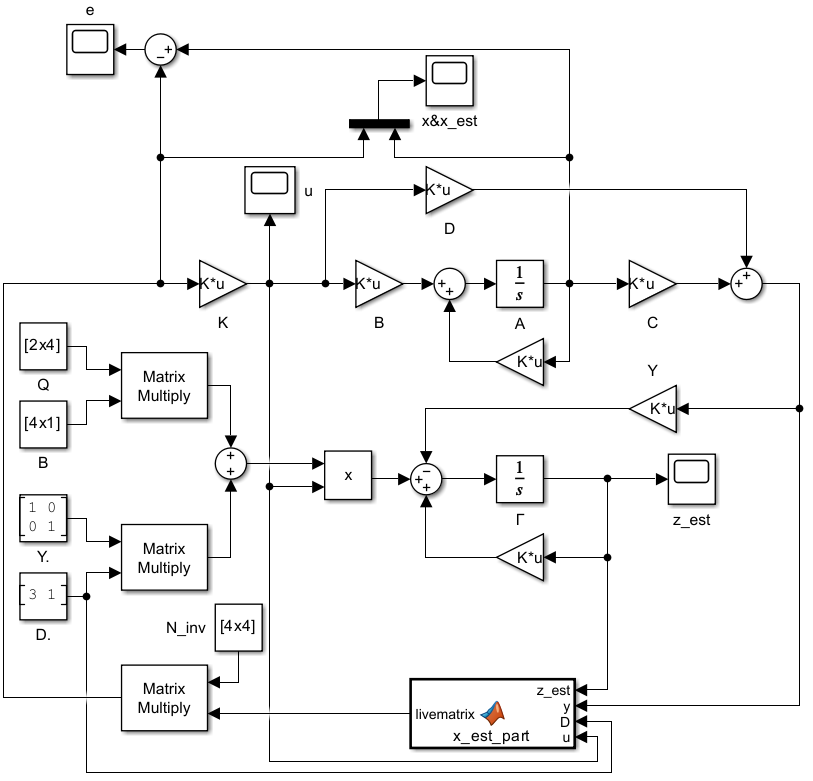
\includegraphics[scale=0.8]{scheme_task4.png}
        \captionsetup{skip=0pt}
        \caption{Схема моделирования системы, замкнутой регулятором, состоящим из наблюдателя состояния пониженного порядка и закона управления}
        \label{fig:scheme_task4}
    \end{figure}


    \subsection{Желаемый спектр матрицы наблюдателя пониженного порядка}
    Для начала определим размерности матриц $\Gamma,Q,Y$. Размерность выхода $k=2$
    -- это измеряемая часть. Порядок системы $n=4$. Тогда
    $$Q_{\left(n-k\right)\times n}\Rightarrow Q_{2\times4},$$
    $$\Gamma_{\left(n-k\right)\times\left(n-k\right)}\Rightarrow\Gamma_{2\times2},$$
    $$Y_{\left(n-k\right)\times k}\Rightarrow Y_{2\times2};$$
    Так как система полностью наблюдаема, то можем задать любой спектр матрицы
    наблюдателя пониженного порядка $\Gamma$. Ограничение -- асимптотическая устойчивость,
    то есть действительные части всех собственных чисел должны быть отрицательными. Пусть
    $$\sigma\left(\Gamma\right)=\left\{-2,-2\right\}\Rightarrow\Gamma=\begin{bmatrix}
        -2 &1\\
        0 &-2
    \end{bmatrix},$$
    $$
    Y=\begin{bmatrix}
        1 &0\\
        0 &1
    \end{bmatrix},\ \text{rank}\begin{bmatrix}
        Y &\Gamma Y
    \end{bmatrix}=\text{rank}\begin{bmatrix}
        1     &0    &-2     &1\\
     0     &1     &0    &-2
    \end{bmatrix}=2;
    $$


    \subsection{Синтез матрицы преобразования}
    Для синтеза матрицы преобразования нужно решить уравнение типа Сильвестра
    $$
    \Gamma Q-QA=YC
    $$
    Предоставим вычисления \texttt{MATLAB}. Получаем
    $$
    Q=\begin{bmatrix}
    -0.0678    &0.2378   &-0.1822   &-0.2622\\
   -0.0667    &0.2667    &0.0667   &-0.2333
    \end{bmatrix}
    $$


    Также найдем матрицу
    $$
    N=\begin{bmatrix}
        C\\Q
    \end{bmatrix},
    $$
    обратная от которой необходима для вычисления $\hat{x}$
    $$
    N=\begin{bmatrix}
    0         &0    &1         &0\\
    1         &0         &0         &0\\
   -0.0678    &0.2378   &-0.1822   &-0.2622\\
   -0.0667    &0.2667    &0.0667   &-0.2333
    \end{bmatrix},
    $$
    $$N^{-1}=\begin{bmatrix}
    0    &1         &0         &0\\
   -4.1538    &0.1154  &-16.1538   &18.1538\\
    1         &0         &0         &0\\
   -4.4615   &-0.1538  &-18.4615   &16.4615
    \end{bmatrix};
    $$


    \subsection{Компьютерное моделирование}
    Выполним компьютерное моделирование, соответствующее схеме \ref{fig:scheme_task4}, с начальными условиями системы
    $x(0)=\begin{bmatrix}
        1 &1 &1 &1
    \end{bmatrix}^T$ и наблюдателя $\hat{z}(0)=\begin{bmatrix}
        0 &0
    \end{bmatrix}^T$. Зададим $K=\begin{bmatrix}-2.3888   &-1.7772    &2.4930   &-1.8840\end{bmatrix}$. Построим графики $u(t),\hat{z}(t),x(t),\hat{x}(t),e(t)$
    \begin{figure}[H]
        \centering
        \begin{subfigure}{0.45\textwidth}
            \centering
            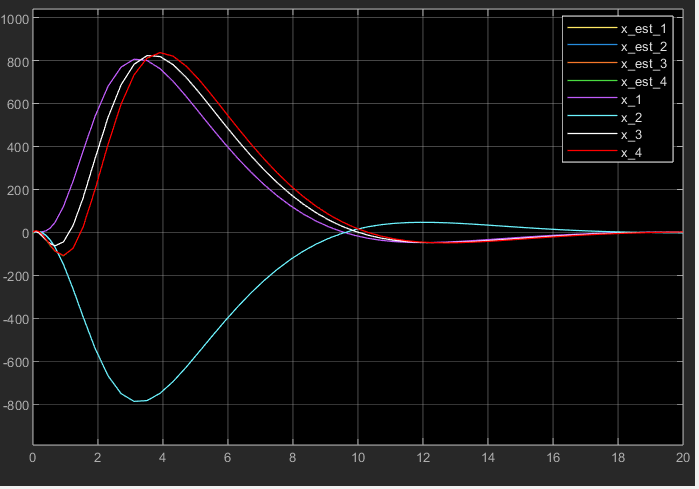
\includegraphics[width=\linewidth]{x_t_x_est_t_task4.png}
            \caption{Графики $x(t),\hat{x}(t)$}
            \label{fig:task_4_x_t}
        \end{subfigure}
        \hfill
        \begin{subfigure}{0.45\textwidth}
            \centering
            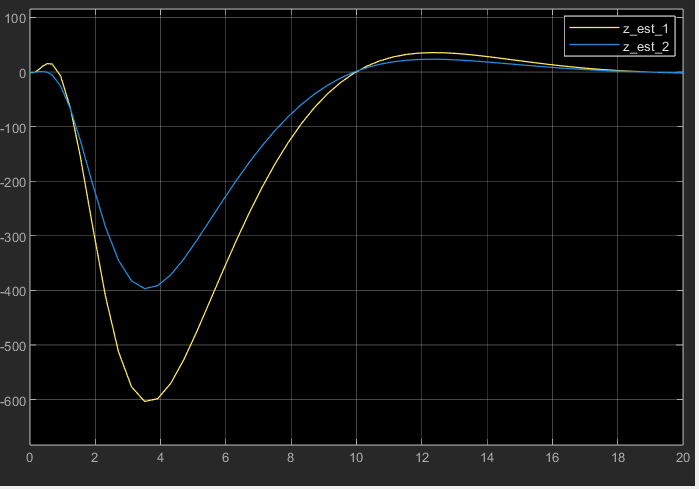
\includegraphics[width=\linewidth]{z_est_t_task4.png}
            \caption{График $\hat{z}(t)$}
            \label{fig:task_4_z}
        \end{subfigure}
        \caption{Графики $x(t),\hat{x}(t),\hat{z}(t)$}
        \label{fig:task_4_modeling}
    \end{figure}
    \begin{figure}[H]
        \centering
        \begin{subfigure}{0.45\textwidth}
            \centering
            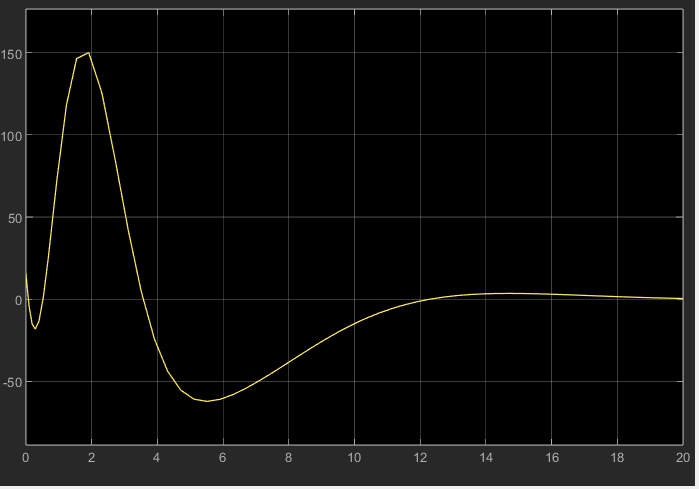
\includegraphics[width=\linewidth]{u_t_task4.png}
            \caption{График $u(t)$}
            \label{fig:u_task_4}
        \end{subfigure}
        \hfill
        \begin{subfigure}{0.45\textwidth}
            \centering
            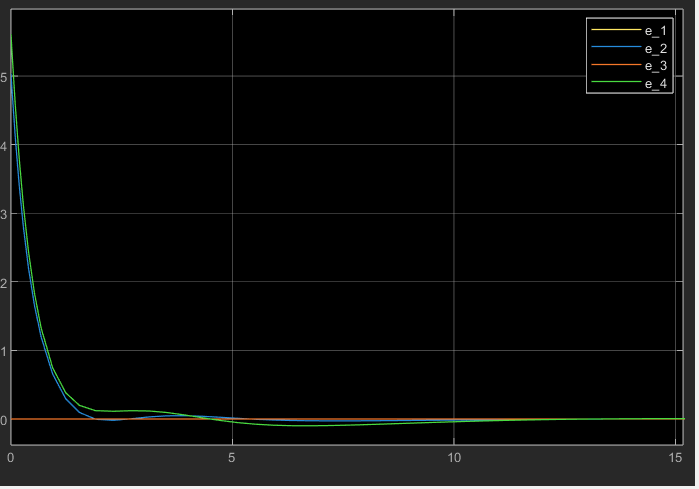
\includegraphics[width=\linewidth]{e_task4.png}
            \caption{График $e(t)$}
            \label{fig:task_4_e}
        \end{subfigure}
        \caption{Графики $u(t),e(t)$}
        \label{fig:task_4_modeling_2}
    \end{figure}
    \noindent Проверим начальные условия
    \begin{figure}[H]
        \centering
        \begin{subfigure}{0.45\textwidth}
            \centering
            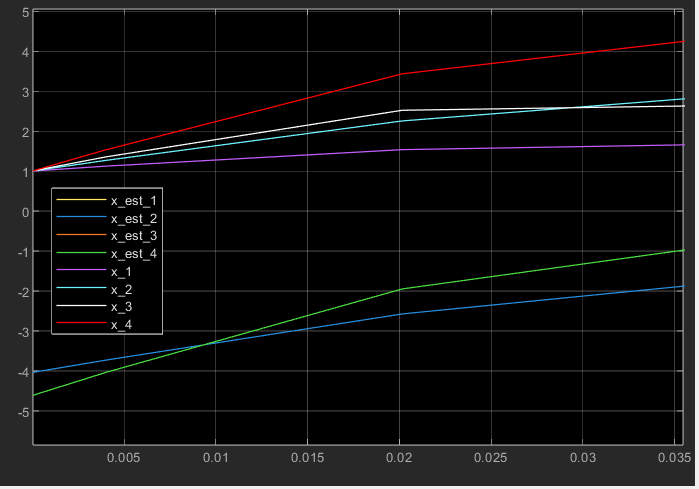
\includegraphics[width=\linewidth]{x_0_x_est_0_task4.png}
            \caption{Графики $x(t),\hat{x}(t)$}
            \label{fig:task_4_x_0_chek}
        \end{subfigure}
        \hfill
        \begin{subfigure}{0.45\textwidth}
            \centering
            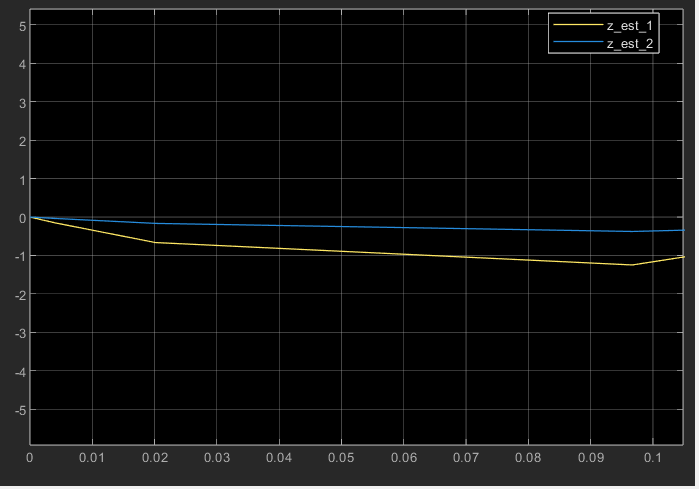
\includegraphics[width=\linewidth]{z_est_0_task4.png}
            \caption{График $\hat{z}(t)$}
            \label{fig:task_4_z_0_check}
        \end{subfigure}
        \caption{Проверка начальных условий $x(t),\hat{x}(t),\hat{z}(t)$}
        \label{fig:task_4_modeling_3}
    \end{figure}


    \subsection{Вывод}
    Система полностью управляема, стабилизируема. Система полностью наблюдаема,
    обнаруживаема. Была найдена матрица преобразования на основании желаемого спектра
    матрицы наблюдателя пониженного порядка. Было выполнено компьютерное моделирование
    с начальными условиями и получены графики формируемого регулятором управления $u(t)$,
    вектора состояния наблюдателя пониженной размерности $\hat{z}(t)$, сравнения $x(t),\hat{x}(t)$,
    а также график ошибки наблюдателя $e(t)$. Начальные условия соблюдены. Ошибка получилась наибольшей в начале, далее
    она плавно стремится к нулю. Графики $x(t),\hat{x}(t)$ сошлись и со временем с некоторого
    момента $t$ стремятся к нулю. Управления также со временем нужно меньше.
    График $\hat{z}(t)$ со временем сходится к нулю.
    

    \section{Общий вывод по работе}
    В данной лабораторной работе мы исследовали модальный регулятор,
    наблюдатель полного порядка, модальное управление по выходу и
    наблюдатель пониженного порядка. Мы определяли управляемость,
    стабилизируемость, наблюдаемость и обнаруживоемость систем.
    На основе этих данных мы задавали желаемые спектры и синтезировали матрицы.
    В конце каждого задания мы моделировали системы. Таким образом, мы убедеждались, что наши
    вычисления и рассуждения верны.


    \section{Приложения}
    \subsection{Приложение 1}
    \begin{lstlisting}[label=task1, caption={Программа для первого задания}]
    % input data
    A = [5 2 7; 2 1 2; -2 -3 -4];
    B = [3; 1; -1];

    % A matrix eigenvalues
    A_e = eig(A);
    disp(A_e);

    % Jordan matrix
    [P, J] = jordan(A);
    Pre(:,1) = P(:,1);
    Pre(:,2) = imag(P(:,2));
    Pre(:,3) = real(P(:,3));
    Pre_inv = Pre^-1; 
    J_re = Pre_inv * A * Pre;
    B_jre = Pre_inv * B;
    disp(Pre);
    disp(Pre_inv);
    disp(J_re);
    disp(B_jre);

    % G matrices
    G1 = [0 1 0; 0 0 1; -8 -12 -6];
    Y1 = [1 0 0];
    O1 = [Y1; Y1*G1; Y1*G1^2];
    rank_O1 = rank(O1);
    disp(O1);
    disp(rank_O1);

    G2 = [0 1 0; 0 0 1; -8000 -4440 -222];
    Y2 = [1 0 0];
    O2 = [Y2; Y2*G2; Y2*G2^2];
    rank_O2 = rank(O2);
    disp(O2);
    disp(rank_O2);

    G3 = [0 1 0; 0 0 1; -80 -48 -6];
    Y3 = [1 0 0];
    O3 = [Y3; Y3*G3; Y3*G3^2];
    rank_O3 = rank(O3);
    disp(O3);
    disp(rank_O3);

    % regulator synthesis
    cvx_begin sdp
    variable P1(3,3)
    variable P2(3,3)
    variable P3(3,3)
    A*P1-P1*G1 == B*Y1;
    A*P2-P2*G2 == B*Y2;
    A*P3-P3*G3 == B*Y3;
    cvx_end

    K1 = -Y1*inv(P1);
    disp(P1);
    disp(K1);

    K2 = -Y2*inv(P2);
    disp(P2);
    disp(K2);

    K3 = -Y3*inv(P3);
    disp(P3);
    disp(K3);

    % A+BK eigenvalues
    ABK1 = A+B*K1;
    ABK2 = A+B*K2;
    ABK3 = A+B*K3;

    ABK1_eig = eig(ABK1);
    ABK2_eig = eig(ABK2);
    ABK3_eig = eig(ABK3);

    disp(ABK1);
    disp(ABK1_eig);

    disp(ABK2);
    disp(ABK2_eig);

    disp(ABK3);
    disp(ABK3_eig);
    \end{lstlisting}


    \subsection{Приложение 2}
    \begin{lstlisting}[label=task2, caption={Программа для второго задания}]
    % input data
    A = [0 1 0 1;
        -26 -7 20 -11;
        0 1 -1 2;
        16 4 -14 8];
    C = [-1 0 1 -1];

    % A matrix eigenvalues
    A_e = eig(A);
    disp(A_e);

    % Jordan matrix
    [P, J] = jordan(A);
    P_re(:,1) = real(P(:,1));
    P_re(:,2) = imag(P(:,2));
    P_re(:,3) = real(P(:,3));
    P_re(:,4) = imag(P(:,4));
    P_re_inv = P_re^-1; 
    J_re = P_re_inv * A * P_re;
    C_jre = C * P_re;
    disp(P_re);
    disp(P_re_inv);
    disp(J_re);
    disp(C_jre);

    % G matrices
    Y = [1; 0; 0; 0];

    G1 = [0 1 0 0; 0 0 1 0; 0 0 0 1; -16 -32 -24 -8];
    U1 = [Y G1*Y G1^2*Y G1^3*Y];
    disp(U1);
    disp(rank(U1));
    disp(eig(G1));

    G2 = [0 1 0 0; 0 0 1 0; 0 0 0 1; -16000000 -8888000 -448440 -2222];
    U2 = [Y G2*Y G2^2*Y G2^3*Y];
    disp(U2);
    disp(rank(U2));
    disp(eig(G2));

    G3 = [0 1 0 0; 0 0 1 0; 0 0 0 1; -260 -132 -49 -8];
    U3 = [Y G3*Y G3^2*Y G3^3*Y];
    disp(U3);
    disp(rank(U3));
    disp(eig(G3));

    % observer synthesis
    cvx_begin sdp
    variable Q1(4,4)
    variable Q2(4,4)
    variable Q3(4,4)
    G1*Q1-Q1*A == Y*C;
    G2*Q2-Q2*A == Y*C;
    G3*Q3-Q3*A == Y*C;
    cvx_end

    L1 = inv(Q1)*Y;
    disp(Q1);
    disp(L1);

    L2 = inv(Q2)*Y;
    disp(Q2);
    disp(L2);

    L3 = inv(Q3)*Y;
    disp(Q3);
    disp(L3);

    % A+LC eigenvalues
    ALC1 = A+L1*C;
    ALC2 = A+L2*C;
    ALC3 = A+L3*C;

    ALC1_eig = eig(ALC1);
    ALC2_eig = eig(ALC2);
    ALC3_eig = eig(ALC3);

    disp(ALC1);
    disp(ALC1_eig);

    disp(ALC2);
    disp(ALC2_eig);

    disp(ALC3);
    disp(ALC3_eig);
    \end{lstlisting}


    \subsection{Приложение 3}
    \begin{lstlisting}[label=task3, caption={Программа для третьего задания}]
    % input data
    A = [2 0 -4 2;
        0 2 -2 4;
        -4 -2 2 0;
        2 4 0 2];
    B = [2;4;6;8];
    C = [-2 2 2 2;
        2 0 0 2];
    D = [3;1];

    % A eigenvalues
    disp(eig(A));

    % controlability
    U = [B A*B A^2*B A^3*B];
    disp(rank(U));

    % observability
    V = [C;C*A;C*A^2;C*A^3];
    disp(rank(V));

    % Jordan matrix
    [P, J] = jordan(A);
    P_inv = inv(P);
    disp(P);
    disp(J);
    disp(P_inv);

    B_new = P_inv*B;
    C_new = C*P;
    disp(B_new);
    disp(C_new);

    % G control
    G_K = [0 1 0 0;
        0 0 1 0;
        0 0 0 1;
        -1 -4 -6 -4];
    Y_K = [1 0 0 0];
    O = [Y_K; Y_K*G_K; Y_K*G_K^2; Y_K*G_K^3];
    disp(O);
    disp(rank(O));

    % regulator synthesis
    cvx_begin sdp
    variable P(4,4)
    A*P-P*G_K == B*Y_K;
    cvx_end

    K = -Y_K*inv(P);
    disp(P);
    disp(K);

    % A+BK eigenvalues
    ABK = A+B*K;
    disp(ABK);
    disp(eig(ABK));

    % G observe
    G_L = [0 1 0 0;
        0 0 1 0;
        0 0 0 1;
        -108 -135 -63 -13];
    Y_L = [1 0;
        0 1;
        0 0;
        0 0];
    U = [Y_L G_L*Y_L G_L^2*Y_L G_L^3*Y_L];
    disp(U);
    disp(rank(U));

    % observer synthesis
    cvx_begin sdp
    variable Q(4,4)
    G_L*Q-Q*A == Y_L*C;
    cvx_end

    L = inv(Q)*Y_L;
    disp(Q);
    disp(L);

    % A+LC eigenvalues
    ALC = A+L*C;
    disp(ALC);
    disp(eig(ALC));
    \end{lstlisting}


    \subsection{Приложение 4}
    \begin{lstlisting}[label=task4, caption={Программа для четвертого задания}]
    % input data
    A = [2 0 -4 2;
        0 2 -2 4;
        -4 -2 2 0;
        2 4 0 2];
    B = [2;4;6;8];
    C = [0 0 1 0;
        1 0 0 0];
    D = [3;1];

    % Jordan matrix
    [P, J] = jordan(A);
    P_inv = inv(P);
    disp(P);
    disp(J);
    disp(P_inv);

    B_new = P_inv*B;
    C_new = C*P;
    disp(B_new);
    disp(C_new);

    % G 2x2, Q 2x4, Y 2x2
    G = [-2 1; 0 -2];
    Y = [1 0; 0 1];
    U = [Y G*Y];
    disp(U);
    disp(rank(U));

    % observer synthesis
    cvx_begin sdp
    variable Q(2,4)
    G*Q-Q*A == Y*C;
    cvx_end
    disp(Q);

    N = [C; Q];
    disp(N);

    N_inv = inv(N);
    disp(N_inv);
    \end{lstlisting}


    \subsection{Приложение 5}
    \begin{lstlisting}[label=task42, caption={Параметры блока \texttt{MATLAB Function} (задание 4)}]
    function livematrix = x_est_part(z_est, y, D, u)
    livematrix = [y - D * u; z_est];
    end
    \end{lstlisting}
\end{document}